\documentclass[a4paper,11pt]{article}
%\documentclass[a4paper,10pt]{scrartcl}

\usepackage{xltxtra}		% XeLaTeX
\usepackage{float}
\usepackage{graphicx}
\usepackage{wrapfig}		% Wrap text around figs
\usepackage{lscape}
\usepackage{rotating}		% Sideways figure
\usepackage{hyperref}		% Hyperlinks
\usepackage{caption}		% Hyperlinks to float top
\usepackage{subcaption}
\usepackage{units}			% dB unit
\usepackage{amsmath}		% math \text{}
\usepackage{inputenc}
\usepackage{color}			% Text colors
\usepackage{geometry}		% Set margins
\usepackage{letltxmacro}	% Safely renew commands (normal \let \renew might cause infinite loops if used on robust commands -- see https://tex.stackexchange.com/questions/47351/can-i-redefine-a-command-to-contain-itself)
\usepackage[backend=biber, style=numeric, %citestyle=authoryear, maxcitenames=1,
			]{biblatex}
\geometry{
  a4paper,
  total={170mm,257mm},
  left=20mm,
  top=20mm,
}

%---		BIBLIOGRAPHY		---%
\bibliography{../bib/primary.bib}
\bibliography{../bib/secondary.bib}
\DefineBibliographyStrings{english}{
  references = {Αναφορές},
}
%\renewcommand*{\bibfont}{\scriptsize}

%-------------------------------------Custom commands----------------------------------------------------------
  \usepackage{amsfonts}
  \def \IN{\mathbb N} \def \IZ{\mathbb Z} \def \IQ{\mathbb Q} \def \IR{\mathbb R} \def \IC{\mathbb C}
  \def \NN{\mathbb N} \def \ZZ{\mathbb Z} \def \QQ{\mathbb Q} \def \RR{\mathbb R} \def \CC{\mathbb C}
  \def \deg{^\circ}
  %-------------------------------GREEK LETTERS DEFINITION-------------------------------------------------------
  \newcommand{\gra}{{\alpha}} \newcommand{\grb}{{\beta}} \newcommand{\grg}{{\gamma}} \newcommand{\grd}{{\delta}}
  \newcommand{\gre}{{\epsilon}} \newcommand{\grz}{{\zeta}} \newcommand{\grh}{{\eta}} \newcommand{\gru}{{\theta}}
  \newcommand{\gri}{{\iota}} \newcommand{\grk}{{\kappa}} \newcommand{\grl}{{\lambda}} \newcommand{\grm}{{\mu}}
  \newcommand{\grn}{{\nu}} \newcommand{\grj}{{\xi}} \newcommand{\gro}{{\rm o}} \newcommand{\grp}{{\pi}}
  \newcommand{\grr}{{\rho}} \newcommand{\grs}{{\sigma}} \newcommand{\grt}{{\tau}} \newcommand{\gry}{{\upsilon}}
  \newcommand{\grf}{{\phi}} \newcommand{\grx}{{\chi}} \newcommand{\grc}{{\psi}} \newcommand{\grv}{{\omega}}
  \newcommand{\grA}{{\rm A}} \newcommand{\grB}{{\rm B}} \newcommand{\grG}{{\Gamma}} \newcommand{\grD}{{\Delta}}
  \newcommand{\grE}{{\rm E}} \newcommand{\grZ}{{\rm Z}} \newcommand{\grH}{{\rm H}} \newcommand{\grU}{{\Theta}}
  \newcommand{\grI}{{\rm I}} \newcommand{\grK}{{\rm K}} \newcommand{\grL}{{\Lambda}} \newcommand{\grM}{{\rm M}}
  \newcommand{\grN}{{\rm N}} \newcommand{\grJ}{{\Xi}} \newcommand{\grO}{{\rm O}} \newcommand{\grP}{{\Pi}}
  \newcommand{\grR}{{\rm R}} \newcommand{\grS}{{\Sigma}} \newcommand{\grT}{{\rm T}} \newcommand{\grY}{{\rm Y}}
  \newcommand{\grF}{{\Phi}} \newcommand{\grX}{{\rm X}} \newcommand{\grC}{{\Psi}} \newcommand{\grV}{{\Omega}}
  %---------------------------------------------------------------------------------------------------------------

\newcommand{\code}[1] {\texttt{#1}}

\setromanfont[Mapping=tex-text]{Linux Libertine O}
\setsansfont[Mapping=tex-text]{DejaVu Sans}
\setmonofont[Mapping=tex-text]{DejaVu Sans Mono}

\renewcommand{\figurename}{Σχήμα}
\renewcommand{\tablename}{Πίνακας}
\renewcommand{\refname}{Αναφορές}

\LetLtxMacro{\oldemph}{\emph}
\renewcommand{\emph}[1]{\textcolor{blue}{\oldemph{#1}}}


\usepackage[section]{placeins}		% Figures in the same section
\let\Oldsection\section
\renewcommand{\section}{\FloatBarrier\Oldsection}	% or subsection
\let\Oldsubsection\subsection
\renewcommand{\subsection}{\FloatBarrier\Oldsubsection}	% or subsection

\title{Προσαρμοστική Μηχανική Μάθηση \linebreak Hierarchical Temporal Memory και νευρομορφικό hardware}
\author{Βασίλειος Αταλόγλου και Κωνσταντίνος Σαμαράς-Τσακίρης}
\date{\today}

\begin{document}
\maketitle

\subsubsection*{Παρατήρηση}
Καθώς το κείμενο αυτό είναι συμπληρωματικό της παρουσίασης, θα γίνονται αναφορές σε αυτή και σε άλλο υλικό όπου αυτό κρίνεται επαρκές. Γενικά προτείνεται να διαβαστεί παράλληλα με την παρουσίαση.

\begin{section}{Hierarchical Temporal Memory}
  \begin{subsection}{Το πρόβλημα της πρόβλεψης ακολουθιών}
	Όπως μας πληροφορεί ο LeCun \cite{lecun}, τα σύνορα της τεχνητής νοημοσύνης ξεπερνούν το πρόβλημα της εκμάθησης ενός στατικού συνόλου δεδομένων με supervised μεθόδους, όπως γίνεται σε πολλές σύγχρονες εφαρμογές. Η τεχνητή νοημοσύνη καλείται σήμερα να αξιοποιήσει τις τεράστιες και συνεχείς ροές δεδομένων που παρέχει το (ανθρωπογενές και μη) περιβάλλον, σε πραγματικό χρόνο, και γενικώς δίχως την πολυτέλεια της προσήμανσης που απαιτεί η επιβλεπόμενη μάθηση.

	Επομένως, καλούμαστε να μοντελοποιήσουμε έναν κόσμο που αλλάζει \cite{staticbottleneck}. Το μοντέλο οφείλει ή να είναι γενικότερο από όλες τις δυνατές μεταβολές του κόσμου ή να αλλάζει μαζί του. Η έννοια της ροής δεδομένων που αναφέρθηκε υπονοεί την έννοια του χρόνου, της αλληλουχίας, που δίνει στο μοντέλο μας ένα νέο εργαλείο: την αιτιώδη σχέση. Την ερμηνεία του κόσμου με τη βοήθεια της συνεπαγωγής και της αναγνώρισης απαιτήσεων και συνεπειών.

	Θεσμοθετείται έτσι το πρόβλημα της εκμάθησης ακολουθιών (sequence learning). Δηλαδή: ο πράκτορας, που παρακολουθεί μια αλληλουχία δεδομένων (γεγονότων), καλείται να \emph{προβλέψει} τη συνέχεια και να \emph{δράσει} έτσι, ώστε να ανταμειφθεί. Η ανταμοιβή, το κίνητρο και γενικότερα ο στόχος, έχει τεθεί από εξωτερικό παράγοντα και βρίσκεται εκτός του πλαισίου της νοημοσύνης. Η παρατήρηση αυτή προσδιορίζει σε κάποιο βαθμό τι εννοείται με τον όρο ``νοημοσύνη'', η οποία δεν αρκεί για τη λειτουργία ενός ζωντανού οργανισμού. Μια άμεση εφαρμογή του προβλήματος της πρόβλεψης είναι και η \emph{αναγνώριση ανωμαλιών}.

	Η εκμάθηση ακολουθιών είναι κλασικό πρόβλημα, για το οποίο έχουν αναπτυχθεί κλασικές λύσεις. Κυριότερο και ευρύτερα διαδεδομένο είδος μοντέλων, ειδικά πριν τη σύγχρονη επάνοδο των νευρωνικών δικτύων, είναι τα Hidden Markov Models. Τα κλασικά (στυλ perceptron) νευρωνικά δίκτυα προσφέρουν στο πρόβλημα τα ``time-delay neural networks'' (TDNN). Η ουσιαστική συνεισφορά των κλασικών νευρωνικών δικτύων επιτυγχάνεται όμως με τα ανάδρομα δίκτυα (recurrent neural networks), που γενίκευσαν τις παλαιότερες feedforward αρχιτεκτονικές ακριβώς για να μπορούν να αντιμετωπίσουν εγγενώς προβλήματα ακολουθιών. Ιδιαίτερης μνείας χρήζει η δομή ``Long short-term memory'' (LSTM). Όλα όμως αυτά τα μοντέλα έχουν σημαντικούς περιορισμούς.

	Ο ανθρώπινος εγκέφαλος, συγκεκριμένα ο φλοιός (neocortex), είναι το βασικότερο παράδειγμα ευφυούς συστήματος που επιλύει το παραπάνω πρόβλημα. Θα ήταν εύλογο λοιπόν να μοντελοποιηθεί η λειτουργία του με αλγοριθμικό τρόπο, που θα στηρίζεται στις βασικές αρχές της εγκεφαλικής λειτουργίας. Για ένα τέτοιο εγχείρημα βεβαίως απαιτείται να γίνει κατανοητό ποια χαρακτηριστικά του εγκεφάλου όντως απαιτούνται για τη λειτουργία του αυτή.

	Ίσως φανούν χρήσιμες μερικές νευρολογικές παρατηρήσεις για τον εγκεφαλικό φλοιό:
	\begin{itemize}
	  \item Η μορφή του είναι διδιάστατη, με τους νευρώνες να ταξιθετούνται σε διακριτά, στοιβαγμένα επίπεδα.
	  \item Η δομή του είναι ομοιόμορφη σε όλη του την έκταση. Μπορεί να θεωρηθεί ότι κάθε περιοχή του neocortex λύνει το ίδιο πρόβλημα με τον ίδιο τρόπο.
	  \item Οι περιοχές ενώνονται ιεραρχικά. Επομένως, οι ιεραρχικά ανώτερες περιοχές υλοποιούν πιο αφηρημένες ιδέες.
	  \item Οι νευρώνες ενεργοποιούνται σποραδικά και πολύ σπάνια. Αν σχηματίσουμε ένα διάνυσμα με την κατάσταση κάθε νευρώνα, το διάνυσμα αυτό θα είναι αραιό (οι περισσότερες θέσεις 0, ανενεργές)
	\end{itemize}
  \end{subsection}

  \begin{subsection}{Sparse Distributed Representations}
	Με βάση την παρατήρηση της αραιής πυροδότησης των νευρώνων στον εγκέφαλο σχεδιάζουμε ένα μεγάλο, αραιό, δυαδικό διάνυσμα που αναπαριστά την πυροδότηση ή μη κάθε νευρώνα της μελετούμενης περιοχής. Μπορεί να θεωρηθεί ότι κάθε περιοχή ανταλλάσσει τέτοια μεγάλα αραιά δυαδικά διανύσματα με τις επόμενες. Ουσιαστικά, αυτά τα αραιά διανύσματα αποτελούν τη ``δομή δεδομένων'' \cite{neuronssynapses,sdrkanerva} του εγκεφάλου. Το ιδιαίτερο χαρακτηριστικό αυτών των διανυσμάτων, λόγω αυτού που αναπαριστούν, είναι ότι κάθε ξεχωριστό bit τους φέρει σημασιολογικό νόημα -- αντίθετα δηλαδή από την κωδικοποίηση ενός γράμματος σε κώδικα ASCII, όπου νόημα φέρει μόνο η πλήρης ``λέξη''. Εξού και το ``distributed'' του ονόματος.

	\subsubsection{Χωρητικότητα SDR}
	Η χωρητικότητα ενός SDR με μέγεθος n και cardinality (πλήθος μονάδων) w είναι το πλήθος των διαφορετικών SDR με αυτή τη μορφή, δηλαδή οι συνδυασμοί των n ανά w: $$ \binom nw= \frac{n!}{w!(n-w)!} $$

	\subsubsection{Συνδυασμοί SDR}
	Διαφάνεια 9.

	\subsubsection{Σύνολα SDR}
	Διαφάνεια 10.

	Επισημαίνεται μονάχα η \emph{σχεδιαστική ελευθερία} που παρέχουν τα SDR. Όσο μεγαλύτερα SDR χρησιμοποιούνται, τόσο αυξάνεται ο χώρος των ενδεχομένων και τόσο πιο απίθανα γίνονται τα λανθασμένα ταιριάσματα.
  \end{subsection}

  \begin{subsection}{Hierarchical Temporal Memory (Numenta) Overview}
	Αξιοποιώντας τις προηγούμενες παρατηρήσεις για τον εγκεφαλικό φλοιό και τις θεμιτές μαθηματικές ιδιότητες των Sparse Distributed Representations μπορεί να μοντελοποιηθεί η λειτουργία του με ένα υπολογιστικό σύστημα. Το βασικό χαρακτηριστικό του συστήματος αυτού είναι η κωδικοποίηση και ανάκληση ακολουθιών, ενώ δομείται ιεραρχικά όπως ο εγκεφαλικός φλοιός, και γι'αυτό καλείται Hierarchical Temporal Memory (HTM). Εδώ βέβαια ο σκοπός του HTM δεν είναι να μοντελοποιήσει τον εγκεφαλικό φλοιό, αλλά με βάση αυτόν να αντιμετωπίσει το πρόβλημα της εκμάθησης ακολουθιών.
	Όλο το σύστημα που περιγράφεται έχει σχεδιαστεί από την εταιρία Numenta \cite{neuronssynapses}.

	Ένα σύστημα HTM λοιπόν αποτελεί ένα τεχνητό νευρωνικό δίκτυο, αλλά βασιζόμενο σε \emph{έννοιες πολύ διαφορετικές} από τα μοντέλα που συνήθως καλούνται τεχνητά νευρωνικά δίκτυα. Παρακάτω αναλύεται η βασική του δομή.

	\subsubsection{Μοντέλο νευρώνα}
	Πρώτα απ'όλα: νευρώνα ονομάζουμε μια δομή που δέχεται σήματα από άλλους νευρώνες και, όταν αυτά πληρούν κάποιες προϋποθέσεις, ενεργοποιείται, για να στείλει σήματα στους επόμενους νευρώνες. Η επαφή 2 νευρώνων καλείται σύναψη.

	Ο βιολογικός νευρώνας (συγκεκριμένα πυραμιδοειδής νευρώνας που απαντά συχνά στο neocortex) είναι ένα σύνθετο στοιχείο, με πολλούς χώρους και διανεμημένες λειτουργίες, που υλοποιούν τις λογικές πράξεις της άθροισης, του πολλαπλασιασμού, της χωρικής και χρονικής ολοκλήρωσης ταυτόχρονα και παράλληλα σε διαφορετικές ομάδες εισόδων. Η κεντρική δομή του νευρώνα, το σώμα, δέχεται ερεθίσματα από το προηγούμενο ιεραρχικά επίπεδο. Αν έρθουν αρκετά τέτοια ερεθίσματα σε σύντομο χρονικό διάστημα ο νευρώνας ενεργοποιείται. Οι πηγές των σημάτων που ο νευρώνας λαμβάνει στο σώμα του ονομάζονται \emph{receptive field} του νευρώνα.
	Περιφερειακά του σώματος υπάρχουν τα δενδριτικά τμήματα, στα οποία υπάρχουν συνάψεις με νευρώνες του ίδιου επιπέδου, που παρέχουν την πληροφορία των συμφραζόμενων. Κάθε τμήμα αυτόνομα δέχεται σήματα και, αν αυτά είναι αρκετά, προκαλείται ένα NMDA spike. Σε αντίθεση με την ενεργοποίηση του σώματος, αυτό γενικά δεν αρκεί για να ενεργοποιήσει ολόκληρο το νευρώνα· θέτει όμως το νευρώνα σε κατάσταση ``επιφυλακής'', διευκολύνοντας τη μετέπειτα ενεργοποίησή του από σωματικά ερεθίσματα.
	Ο νευρώνας επίσης λαμβάνει ερεθίσματα από την πλευρά του άξονα, από τους νευρώνες δηλαδή που ``δέχονται'' το σήμα του στην κανονική του πορεία. Αυτά αποτελούν σήματα ανάδρασης.

	Μια απλοποιημένη εκδοχή αυτής της περιγραφής αποτελεί και ο υπολογιστικός νευρώνας του συστήματος που επιδεικνύεται. Έχει πάλι 3 περιοχές που συμπεριφέρονται διαφορετικά για να λαμβάνει εισόδους feedforward, context και feedback όπως ο βιολογικός. Επαρκής feedforward είσοδος αρκεί για να τον ενεργοποιήσει, ενώ επαρκής είσοδος context ή feedback τον θέτει στο λεγόμενο ``predictive state''. Αν στη συνέχεια (στη συνέχεια... ακολουθία... συνεπαγωγή...) έρθει feedforward είσοδος, θα ενεργοποιηθεί πιο εύκολα και γρήγορα απ'ό,τι άλλοι νευρώνες με την ίδια είσοδο.
	Σε αντιπαραβολή, ο ``νευρώνας'' ενός κλασικού τεχνητού νευρωνικού δικτύου δεν έχει διακριτά λειτουργικά τμήματα και απλώς αθροίζει όλες τις εισόδους του.

	\subsubsection{Μοντέλο δικτύου}
	Και μόνο ο παραπάνω ανάδρομος ορισμός του νευρώνα παραπέμπει στο ρόλο του ως μονάδα δικτύου.

	Η πρώτη οργανωτική δομή νευρώνων, τόσο στο neocortex, όσο και στο HTM, είναι το minicolumn. Συνοπτικά, ο ρόλος των minicolumns είναι να επιτρέπουν διαφορετικές εσωτερικές αναπαραστάσεις των εξωτερικών (feedforward) ερεθισμάτων, ανάλογα με τα συμφραζόμενα. Όλοι οι νευρώνες του minicolumn μοιράζονται \emph{το ίδιο receptive field}, ενώ μεταξύ τους υπάρχει \emph{inhibition}. Έτσι υλοποιείται μια αρχιτεκτονική ``winner-takes-all'', όπου, αν κάποιοι νευρώνες είναι ήδη σε predictive κατάσταση όταν έρθει feedforward είσοδος που ερεθίζει το minicolumn, θα ενεργοποιηθούν πρώτοι και θα αποτρέψουν την ενεργοποίηση των υπολοίπων.
	Η παραπάνω περιγραφή βέβαια προτρέχει λίγο.

	Πολλά minicolumns συνθέτουν ένα cortical layer, που αποτελεί τη λειτουργική μονάδα ενός συστήματος HTM. Κάθε minicolumn του cortical layer έχει διαφορετικές feedforward συνδέσεις προς την είσοδο του layer, ενώ διαφορετικά minicolumns μοιράζονται μεταξύ τους συνδέσεις που φέρουν πληροφορίες συμφραζομένων. Σε πολλές περιπτώσεις μπορεί να υπάρχει ολικό inhibition μεταξύ των minicolumns. Αν βέβαια το cortical layer έχει κάποια τοπολογική διάταξη προς την είσοδό του\footnote{Δες το βίντεο ``Topology (Episode 10)'' της σειράς ``HTM School'' \cite{htmschool}}, όπως συχνά συμβαίνει στον εγκεφαλικό φλοιό, τότε οι inhibitory συνδέσεις είναι τοπικές και ένα minicolumn δεν ανταγωνίζεται κάποιο άλλο που βρίσκεται μακριά του.
	Τα λειτουργκά παραδείγματα παρακάτω αποτελούνται από 1 cortical layer. Ένα πιο σύνθετο σύστημα θα μπορούσε να ενώσει εν σειρά πολλά cortical layers.

	Οι συνάψεις των HTM νευρώνων είναι επίσης πιστότερες στη βιολογία. Δε χρησιμοποιούν κάποιο βάρος που πολλαπλασιάζει την είσοδο, αλλά είναι δισταθείς, δηλαδή υπάρχουν ή όχι. Ένα μέγεθος όμως που χαρακτηρίζει κάθε σύναψη είναι η \emph{μονιμότητά} της, που διαμορφώνεται δυναμικά από τη μαθησιακή διαδικασία (στην οποία δε θα αναφερθούμε παραπάνω εδώ) με αλγόριθμο τύπου Spike Timing Dependent Plasticity (STDP), που μπορεί ουσιαστικά να εμφανίσει και να εξαφανίσει υποθάλπουσες συνάψεις για να προσαρμόσει το σύστημα στα δεδομένα. Η μονιμότητα μιας σύναψης συγκρίνεται με ένα κατώφλι και, αν είναι πιο πάνω είναι ενεργή, αν είναι πιο κάτω είναι ανενεργή. Μια σύναψη με μονιμότητα λίγο πάνω από το κατώφλι μπορεί δηλαδή να απενεργοποιηθεί εύκολα.

	\subsubsection{Encoders}
	Ο εγκέφαλος έχει ως βασική διεπαφή με τον έξω κόσμο τον αμφιβληστροειδή χιτώνα του ματιού και τον κοχλία του αυτιού. Και τα 2 αυτά συστήματα μπορούμε να θεωρήσουμε ότι μετατρέπουν τα φυσικά ερεθίσματα του κόσμου σε μια πρώτη μορφή SDR, για να ερεθίσουν με τη σειρά τους το επόμενο επίπεδο νευρώνων. Το ρόλο αυτό στα συστήματα HTM καλύπτουν οι encoders.

	Οι encoders μπορεί να είναι από πολύ απλά έως εξαιρετικά πολύπλοκα συστήματα (βλέπε αμφιβληστροειδή). Στη διαφάνεια 13 δίνεται το παράδειγμα ενός απλού encoder που κωδικοποιεί ακέραιους αριθμούς συγκεκριμένου εύρους. Μπορεί όμως να σχεδιαστεί και encoder που να κωδικοποιεί λέξεις ή και κείμενα, όπως κάνει η εταιρία cortical.io \cite{semantic} στη διαφάνεια 14.
  \end{subsection}

  \begin{subsection}{Βασικές λειτουργίες HTM}
	Παρουσιάζονται ένα σύστημα που κανονικοποιεί τα SDR εισόδου, ο \emph{Spatial Pooler}, και ένα σύστημα που μαθαίνει να αναγνωρίζει ακολουθίες απλών ερεθισμάτων, δηλαδή μια \emph{μνήμη ακολουθιών}. Για το πρώτο προτείνονται τα σχετικά βίντεο από τη σειρά ``HTM School'' στο youtube, ενώ για το δεύτερο η αναφορά [2]. Λίγα λόγια για τη μνήμη ακολουθιών:

	\subsubsection{Sequence Memory}
	Στη \emph{διαφάνεια 17} \cite{continuous} βλέπουμε ένα cortical layer που αποτελείται από από minicolumns. Στη μέση (C) βλέπουμε πώς αντιδρά το σύστημα καθώς δέχεται για πρώτη φορά τις αλληλουχίες ``ABCD'' και ``XBCY''. Παρατηρούμε ότι κάθε σύμβολο εισόδου ενεργοποιεί συγκεκριμένα minicolumns (αυτά που διεγείρονται περισσότερο), και ότι σε κάθε τέτοιο minicolumn ενεργοποιούνται \emph{όλοι} οι νευρώνες.

	Ας επικεντρωθούμε στο τι συμβαίνει όταν λαμβάνεται η είσοδος ``A''. Ενεργοποιούνται τα minicolumns που φαίνονται, αλλά κάποιοι από τους ενεργοποιημένους νευρώνες έχουν context συνάψεις (ενεργές ή μη) με κάποιους νευρώνες που ενεργοποιεί η είσοδος ``B''. Αυτό φαίνεται στη διαφάνεια 18 Α. Αφού το σύστημα δει την αλληλουχία A -> B μερικές φορές, συνάψεις αυτού του τύπου ενεργοποιούνται μέσω της διαδικασίας εκμάθησης, ακόμα κι αν στην αρχή ήταν ανενεργές. Έτσι, όταν ξαναέρθει η είσοδος ``A'', συγκεκριμένοι νευρώνες των στηλών που αντιστοιχούν στο ``B'' τίθενται σε predictive state. Όταν λοιπόν όντως έρχεται η είσοδος ``B'' αμέσως μετά αυτοί οι νευρώνες ενεργοποιούνται πρώτοι και μπλοκάρουν μέσω inhibitory συνδέσεων τους υπόλοιπους του ιδίου minicolumn. Έτσι καταλήγουμε στην ακολουθία της κάτω σειράς (D) της διαφάνειας 17. Τα παραπάνω σημαίνουν ότι το σύστημα \emph{προβλέπει την επόμενη είσοδό του}, που είναι ο βασικός στόχος του προβλήματος εκμάθησης ακολουθιών.

	Ο μηχανισμός αυτός οδηγεί σε δύο παρατηρήσεις: η εσωτερική αναπαράσταση κάθε συμβόλου είναι \emph{διαφορετική ανάλογα με τα συμφραζόμενα} και το σύστημα μπορεί να πραγματοποιεί \emph{πολλαπλές προβλέψεις ταυτόχρονα}.

	Το πρώτο φαίνεται στην κάτω σειρά (D) από τους διαφορετικούς νευρώνες που ενεργοποιούνται για να συμβολίσουν την ίδια είσοδο ``B'', ανάλογα αν το προηγούμενο σύμβολο ήταν ``A'' ή ``X'', οπότε προκύπτει η εσωτερική αναπαράσταση B' ή B'' αντίστοιχα.
	Το δεύτερο σημείο φαίνεται στη διαφάνεια 18 Β, όπου δίνεται η είσοδος ``B'', χωρίς να έχει προηγηθεί ``Α'' ή ``Χ''. Το σύστημα τότε προβλέπει την ένωση των 2 καταστάσεων C' και C'', οι οποίες ενεργοποιούνται παράλληλα όταν όντως έρχεται η είσοδος C. Εκείνη τη στιγμή λοιπόν το σύστημα σωστά προβλέπει ότι η συνέχεια της ακολουθίας θα είναι ή ``D'' ή ``Y''.
  \end{subsection}

  \begin{subsection}{Αποτελέσματα - Προσομοιώσεις}
    To ΗΤΜ δοκιμάστηκε τόσο σε τεχνητά, όσο και σε πραγματικά δεδομένα για να αξιολογηθεί η δυνατότητα του να παρέχει ακριβείς προβλέψεις. Παρακάτω θα αναλυθούν δύο παραδείγματα και θα δοθούν τα συγκριτικά διαγράμματα των επιδόσεων με άλλα νευρωνικά δίκτυα.
    \subsubsection{Πρόβλεψη συμβόλου ακολουθίας}
    Οι αλγόριθμοι του Hierarchical Temporal Memory (HTM) δοκιμάστηκαν σε διαφορετικά προβλήματα \cite{continuous,nab}, ώστε να αξιολογηθεί η επίδοση του συστήματος σε σχέση με άλλες υλοποιήσεις. Στο πρώτο παράδειγμα έχουν δημιουργηθεί δύο ακολουθίες από σύμβολα, σύμφωνα με την εικόνα \eqref{fig:sequences}. Στόχος είναι η πρόβλεψη του τελευταίου συμβόλου.
    \begin{figure}[H]
      \centering%
      {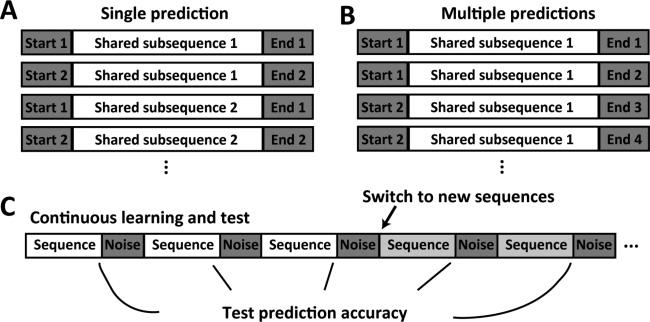
\includegraphics[width=0.8\columnwidth,clip=true]{pics/sequences.jpg}}
      \caption{Ακολουθίες συμβόλων για την προσομοίωση} \label{fig:sequences}
    \end{figure}
    Οι ακολουθίες φτιάχτηκαν έτσι ώστε να χρειάζεται ένα βάθος μνήμης τουλάχιστον 2 παρελθοντικών συμβόλων για την επιτυχή πρόβλεψη. Το πρώτο set ακολουθιών έχει δημιουργηθεί για να ελεγχθεί η δυνατότητα απλής πρόβλεψης, καθώς κάθε ακολουθία προσδιορίζεται πλήρως από τα πεδία ``Start'' και ``Shared Subsequence''. Αντιθέτως, στο δεύτερο set δύο ακολουθίες μπορεί να έχουν ίδια τα παραπάνω πεδία. Σε αυτή την περίπτωση το νευρωνικό δίκτυο θα πρέπει να επιτύχει την ορθή πρόβλεψη όλων των πιθανών καταλήξεων, δηλαδή την ταυτόχρονη πολλαπλή πρόβλεψη. Τέλος, ανάμεσα στις ακολουθίες προστέθηκε ένα σύμβολο θορύβου, ώστε να εξεταστεί η ανθεκτικότητα του συστήματος σε αυτόν.
    \begin{figure}[H]
      \centering%
      {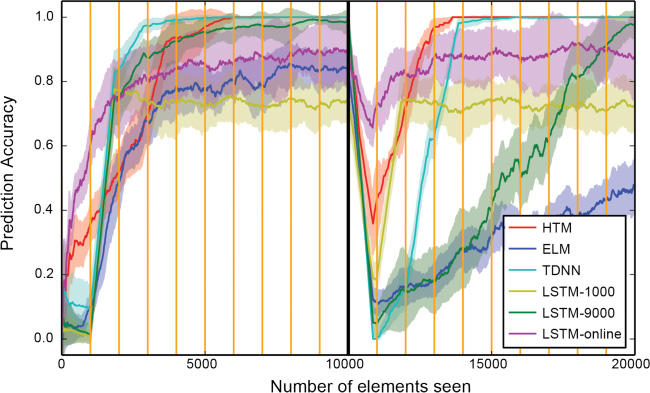
\includegraphics[width=0.7\columnwidth,clip=true]{pics/single_prediction.jpg}}
      \caption{Απόδοση διαφορετικών υλοποιήσεων για απλή πρόβλεψη} \label{fig:single-prediction}
    \end{figure}
    Στο σχήμα \eqref{fig:single-prediction} δίνεται η συγκριτική απόδοση των διαφορετικών υλοποιήσεων νευρωνικών δικτύων για το πρώτο set ακολουθιών. Τα δίκτυα που υλοποιούνται είναι το HTM, το ELM, το TDNN και το LSTM. Ο προσδιορισμός στο LSTM αφορά το πλήθος των δειγμάτων που χρησιμοποιούνται για retraining σε κάθε κατακόρυφη κίτρινη γραμμή του διαγράμματος. Στο στοιχείο 10000 που σημειώνεται με κάθετη κατακόρυφη γραμμή, αλλάζουν αμοιβαία τα δύο τελευταία σύμβολα κάθε ακολουθίας και μελετάται η προσαρμογή του δικτύου στο νέο input space. Βλέπουμε ότι το HTM πετυχαίνει αρχικά σε έναν ικανοποιητικό αριθμό δειγμάτων ακρίβεια $100\%$. Το πιο σημαντικό είναι, βέβαια, ότι μέσω online training αναπροσαρμόζεται ταχύτερα από κάθε άλλη υλοποίηση στο νέο χώρο ακολουθιών εισόδου.\\
    \begin{figure}[H]
      \centering%
      {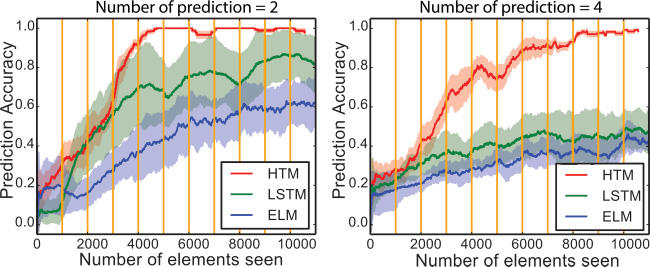
\includegraphics[width=0.8\columnwidth,clip=true]{pics/multiple_predictions.jpg}}
      \caption{Απόδοση δικτύων για πολλαπλές προβλέψεις} \label{fig:multiple-prediction}
    \end{figure}
    Οι πολλαπλές προβλέψεις εξετάζονται από το δεύτερο σετ και τα συγκριτικά αποτελέσματα για διπλή και τετραπλή πρόβλεψη δίνεται στο σχήμα \eqref{fig:multiple-prediction}. Όπως φαίνεται, το HTM είναι το μοναδικό σύστημα που πετυχαίνει μετά από κάποιο διάστημα ακρίβεια σχεδόν $100\%$. Αυτό απορρέει από την αναπαράσταση μέσω SDR και τη δυνατότητα του Temporal Pooler για πολλαπλές προβλέψεις.\\
    Στη συνέχεια, μελετήθηκε η απόδοση του HTM για ακολουθίες διαφορετικού μήκους. Ένα από τα τα σημαντικότερα στοιχεία του Temporal Pooler είναι η δυνατότητα αναπροσαρμογής online του «βάθους» μνήμης που χρησιμοποιείται για την πρόβλεψη. Έτσι, όπως παρατηρούμε και στο διάγραμμα \eqref{fig:sequence-order}, πετυχαίνει πρόβλεψη ακόμα και τάξης 100, που σημαίνει ότι απαιτείται μνήμη 99 συμβόλων για να προβλεφθεί επιτυχώς το τελευταίο. Το πλήθος των ακολουθιών που απαιτείται για να εκπαιδευτεί το σύστημα και να πετύχει ακρίβεια κοντά στο $100\%$ αυξάνει γραμμικά με την τάξη της ακολουθίας.
    \begin{figure}[H]
      \centering%
      {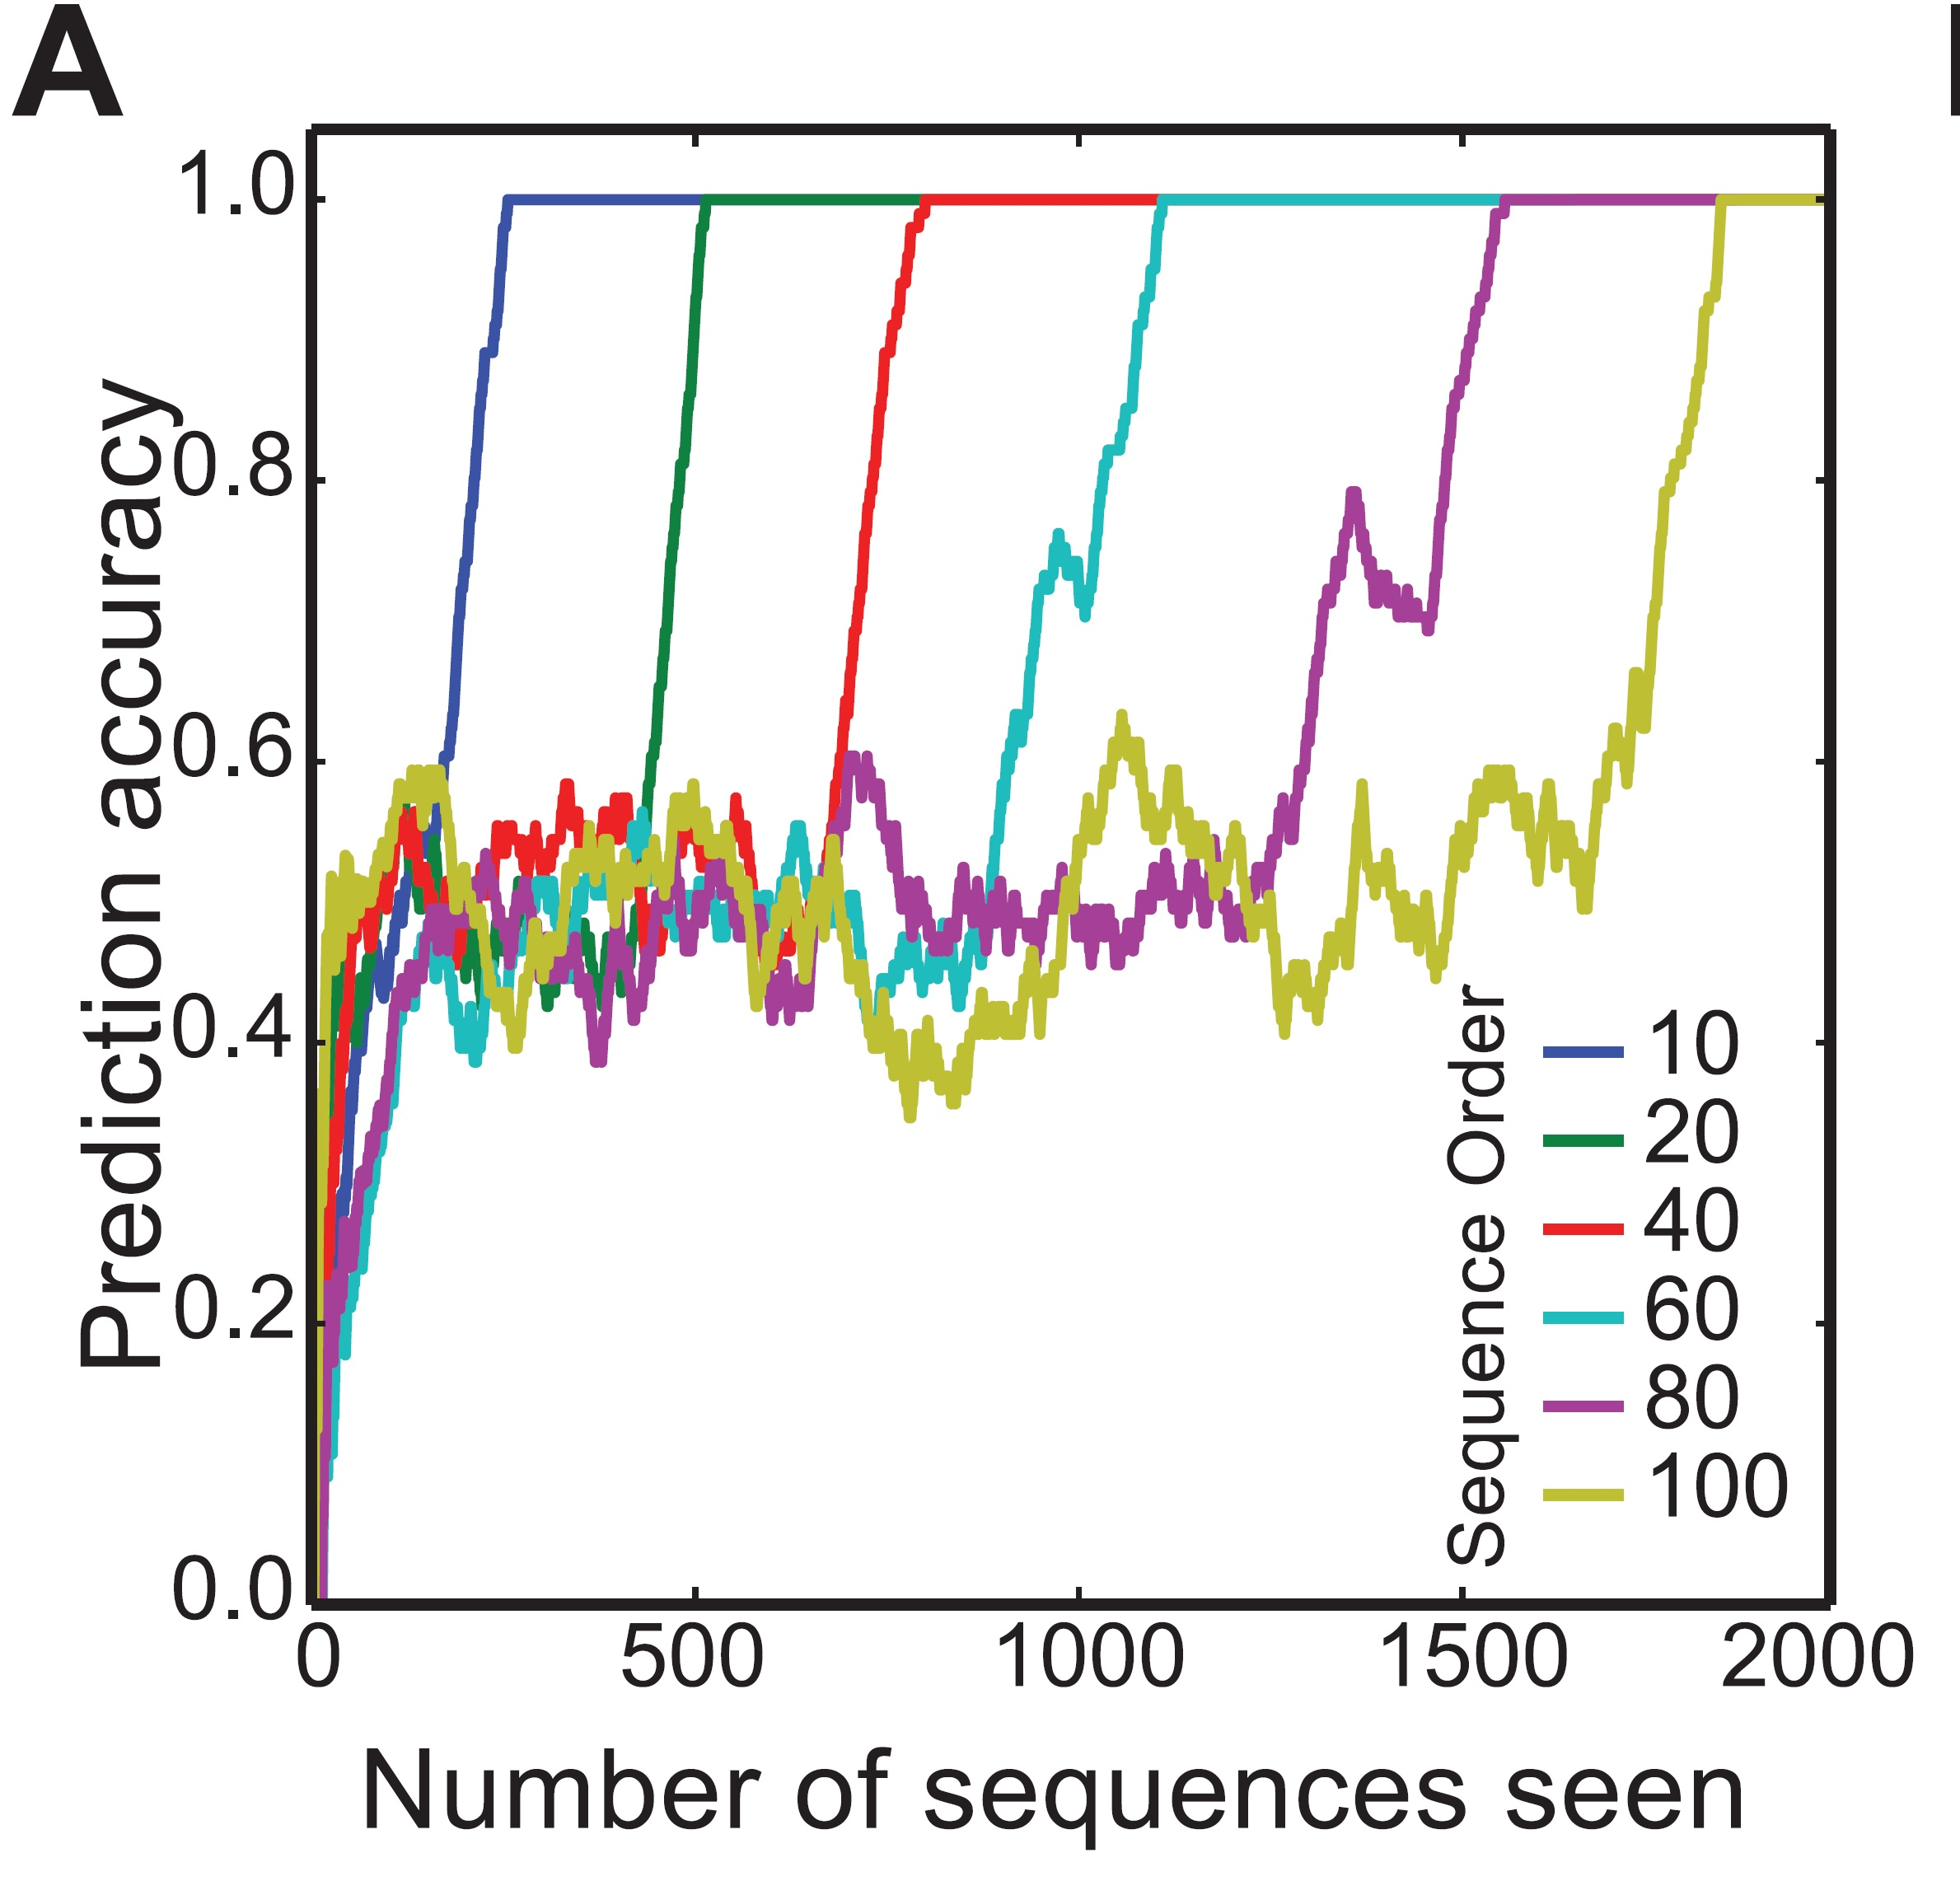
\includegraphics[width=0.4\columnwidth,clip=true]{pics/sequence_order.jpg}}
      \caption{Απόδοση HTM συναρτήσει της τάξης της ακολουθίας} \label{fig:sequence-order}
    \end{figure}
    Τέλος, τα διαφορετικά συστήματα εξετάστηκαν και ως προς την ανθεκτικότητα σε καταστροφή του δικτύου μέσω νεκρών νευρώνων. Το HTM έμεινε ανεπηρέαστο ακόμα για $30\%$ νεκρούς νευρώνες, συνθήκες κατά τις οποίες το ELM και το LSTM είχαν υποβαθμιστεί αρκετά.
    \begin{figure}[H]
      \centering%
      {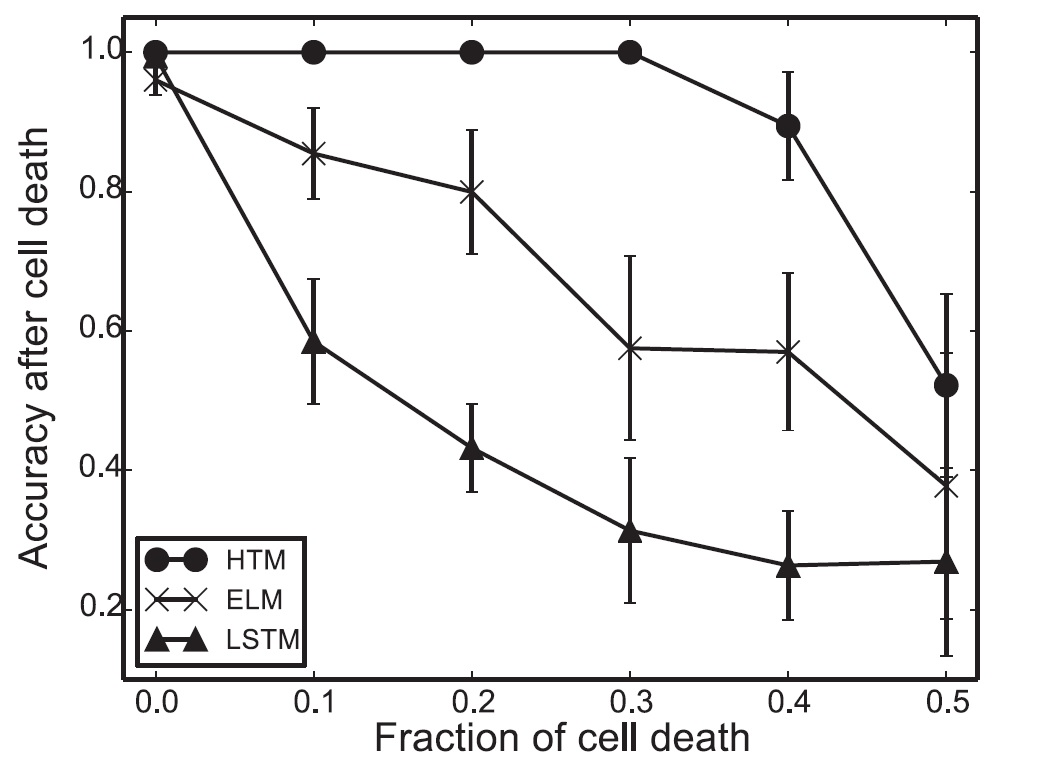
\includegraphics[width=0.4\columnwidth,clip=true]{pics/cell_death.jpg}}
      \caption{Ανθεκτικότητα υλοποιήσεων σε νεκρούς νευρώνες} \label{fig:cell-death}
    \end{figure}


    \subsubsection{Πρόβλεψη της ζήτησης taxi στη Νέα Υόρκη}

    Το Hierarchical Temporal Memory δοκιμάστηκε και σε πραγματικά streaming δεδομένα. Πιο συγκεκριμένα, ζητήθηκε η πρόβλεψη της ζήτησης στα taxi της Νέας Υόρκης 2.5 ώρες πριν την πραγματική μέτρηση. Η ζήτηση ποσοτικοποιήθηκε ως η συνολική εξυπηρέτηση πελατών σε ένα χρονικό παράθυρο 30 λεπτών. Εξετάστηκαν διάφοροι τύποι νευρωνικών δικτύων, καθώς και το στατιστικό μοντέλο ARIMA. Όπως παρατηρούμε από την εικόνα \eqref{fig:taxi_accuracy}, το HTM πέτυχε το μικρότερο απόλυτο σφάλμα πρόβλεψης (της τάξης του $0.08\%$ ).\\
    \begin{figure} [H]
      \centering%
      \begin{subfigure}{0.5\columnwidth}
        {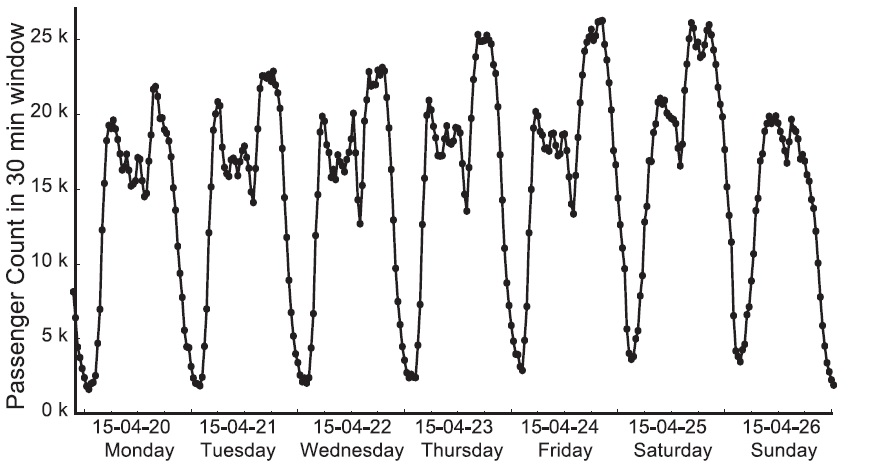
\includegraphics[width=\columnwidth,clip=true]{pics/taxi_demand.jpg}}
        \caption{Διάγραμμα ζήτησης}\label{fig:taxi_demand}
      \end{subfigure}%
      \begin{subfigure}{0.5\columnwidth}
        \centering
        {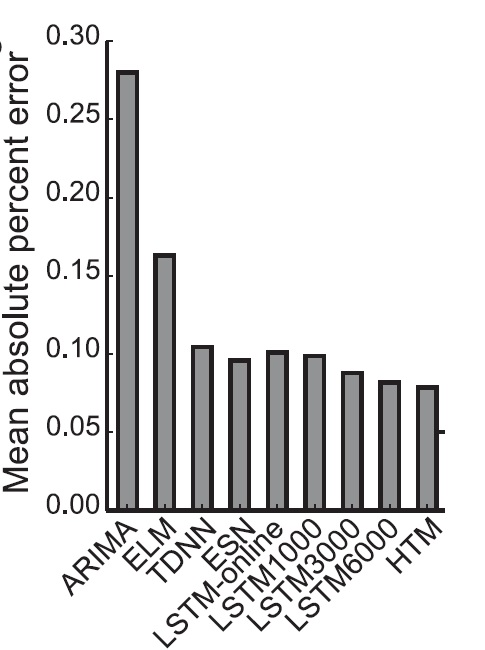
\includegraphics[width=0.5\columnwidth,clip=true]{pics/taxi_accuracy.jpg}}
        \caption{Μέσο απόλυτο σφάλμα}\label{fig:taxi_accuracy}
      \end{subfigure} \label{fig:taxi_simulation}
      \caption{Πρόβλεψη ζήτησης των taxi}
    \end{figure}

    Στη συνέχεια, τα δεδομένα εισόδου τροποποιήθηκαν τεχνητά ανεβάζοντας ή μειώνοντας τη ζήτηση κατά $20\%$ σε διαφορετικές χρονικές περιόδους εντός κάθε μέρας. Στόχος ήταν να μελετηθεί η προσαρμογή του δικτύου στις νέες (τεχνητές) συνήθειες των επιβατών taxi της Νέας Υόρκης. Η αλλαγή πραγματοποιήθηκε την 1η Απριλίου και εντός 2 βδομάδων το σύστημα HTM αναπροσάρμοσε το μοντέλο του, ώστε να πετυχαίνει εκ νέου σωστές προβλέψεις. Σε αντίθεση, το LSTM είτε απέτυχε να επανέρθει, είτε χρειάστηκε πολύ περισσότερο διάστημα για retraining των παραμέτρων του.
    \begin{figure}[h]
      \centering%
      {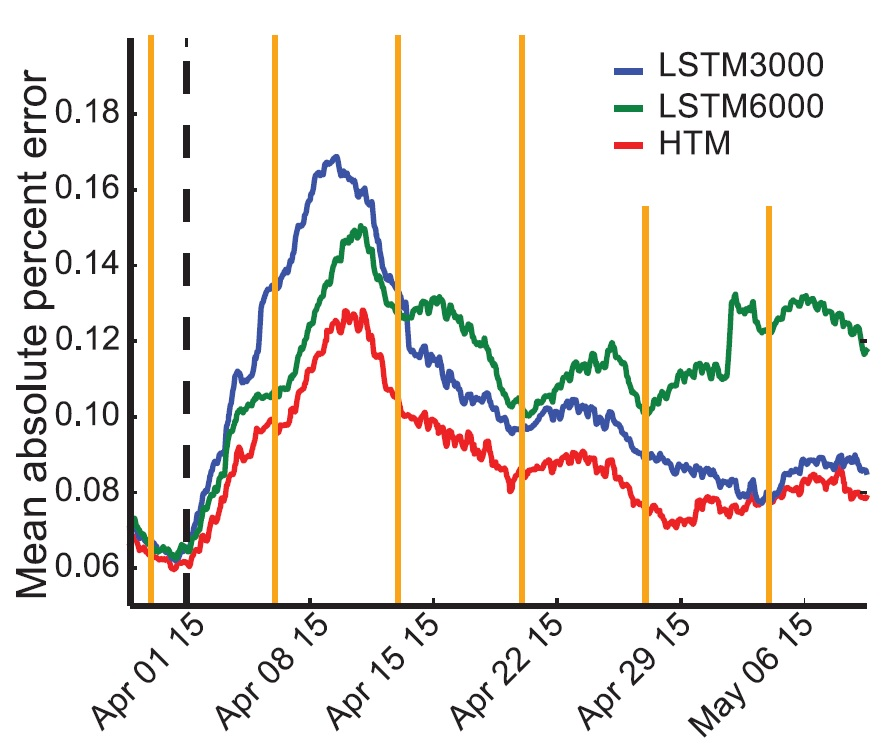
\includegraphics[width=0.4\columnwidth,clip=true]{pics/taxi_adaptation.jpg}}
      \caption{Προσαρμογή δικτύων σε μεταβολή της ζήτησης} \label{fig:taxi-adaptation}
    \end{figure}

  \end{subsection}
\end{section}

\pagebreak
\begin{section}{Neuromorphic processors and hardware HTM}
  \begin{subsection}{SpiNNaker}
    Το SpiNNaker (Spiking Neural Network Architecture) είναι ένα ψηφιακό υπολογιστικό σύστημα υψηλής παραλληλοποίησης κατάλληλο μοντελοποίηση νευρωνικών δικτύων. Αναπτύχθηκε από το Πανεπιστήμιο του Manchester με σκοπό να προσομοιώσει μέρος του ανθρώπινου εγκεφάλου (συγκεκριμένα το $1\%$ των νευρώνων)
    \subsubsection{Αρχιτεκτονική Συστήματος}

    Βασικό δομικό στοιχείο του SpiNNaker είναι το SpiNNaker Multiprocessor Chip (CMP). Πρόκεται για chip που απολείται από 18 σύγχρονους ARM968 processors που επικοινωνούν μεταξύ τους ασύγχρονα. Είναι κατασκευασμένο σε τεχνολογία CMOS $130nm$, λειτουργεί στα $180ΜHz$ και καταναλώνει μόλις $1W$.
    \begin{figure} [H]
      \centering%
      \begin{subfigure}{0.5\columnwidth}
        \centering
        {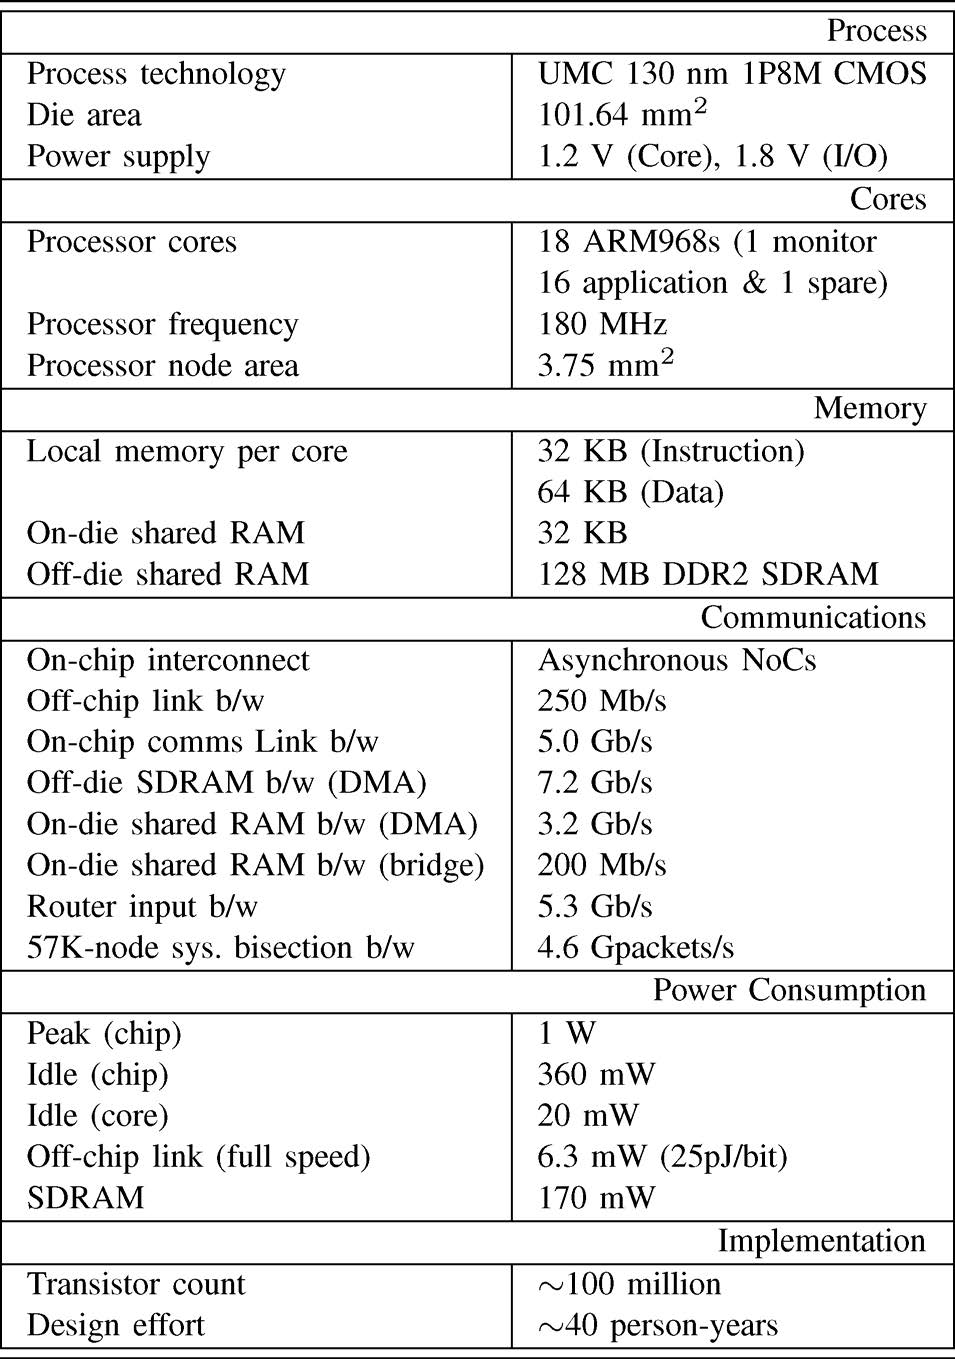
\includegraphics[width=0.8\columnwidth,clip=true]{pics/CMPspecs.jpg}}
        \caption{CMP specifications}\label{fig:CMP-specs}
      \end{subfigure}%
      \begin{subfigure}{0.5\columnwidth}
        \centering
        {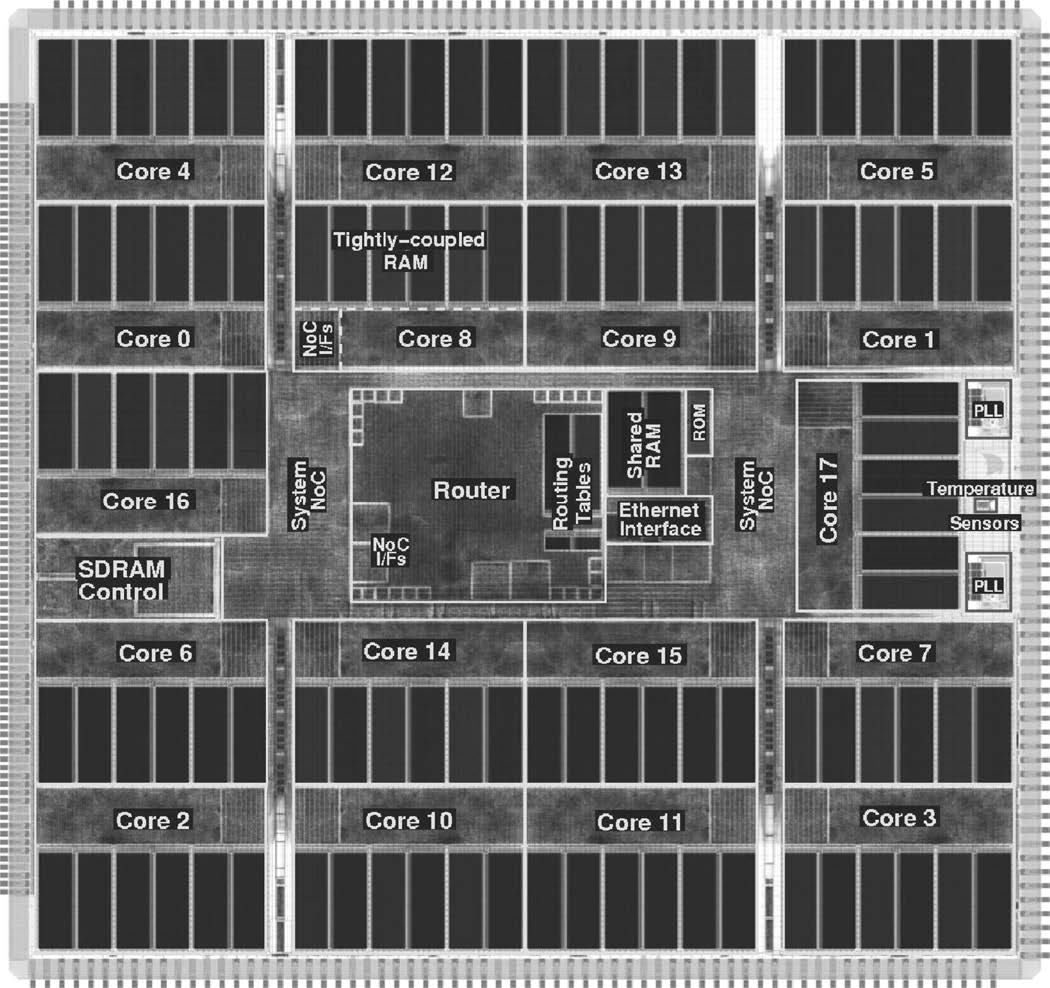
\includegraphics[width=0.9\columnwidth,clip=true]{pics/CMP.jpg}}
        \caption{Πλακίδιο CMP}\label{fig:CMP-die}
      \end{subfigure}
      \caption{SpiNNaker Multiprocessor Chip (CMP)}
    \end{figure}

    Το συνολικό σύστημα αποτελείται από κόμβους που περιέχουν ένα CMP και ένα στοιχείο SDRAM μέσα σε ένα κοινό package. Στην τελευταία ολοκληρωμένη υλοποίηση, υπάρχουν 57600 κόμβοι που περιέχουν συνολικά $10^6$ ARM968. Κάθε ΑRM μπορεί να μοντελοποιήσει περίπου 1000 νευρώνες. Αυτό το πλήθος, βέβαια, μπορεί να ποικίλλει ανάλογα με την πολυπλοκότητα του μοντέλου που χρησιμοποιείται για το νευρώνα. Συνολικά, έχουμε δηλαδή $10^9$ νευρώνες που αποτελούν το $1\%$ του ανθρώπινου εγκεφάλου. Η υπολογιστική ισχύς είναι της τάξης των 228 TIPS. Ενδεικτικά, ένας τελευταίας γενιάς i7 της Intel πετυχαίνει περίπου 300GIPS.\\
    Άξια σχολιασμού είναι φυσικά και η κατανάλωση ισχύος ενός τέτοιου μηχανήματος. Παρά τις προσπάθειες για την ελαχιστοποίηση της, το SpiNNaker καταναλώνει περίπου 90ΚW. Συγκρίνοντας με τα 25W του ανθρώπινου εγκεφάλου, φαίνεται ακόμη περισσότερο το μεγαλείο αυτής της ((μηχανής)) που βιολογικά έχει εξελιχθεί κατά τη διάρκεια ύπαρξης του ανθρώπινου είδους.\\
    \begin{figure}[H]
      \centering%
      {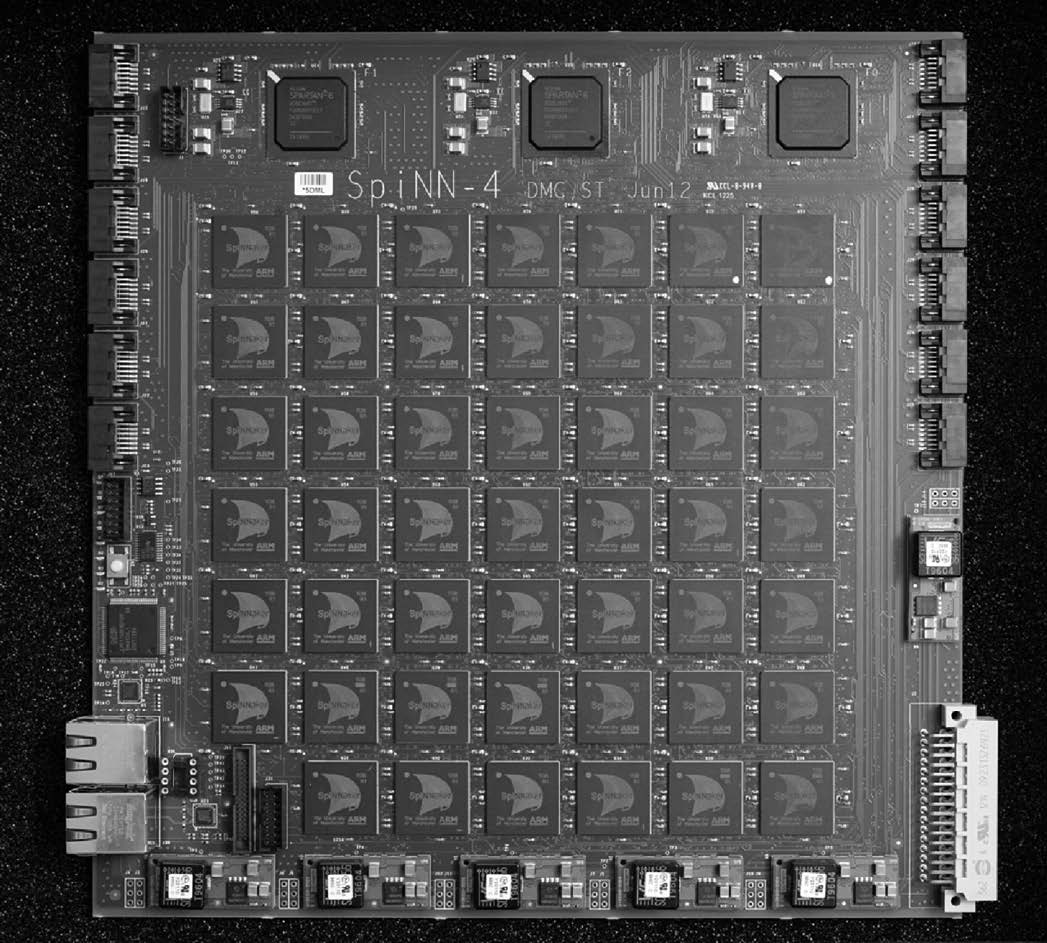
\includegraphics[width=0.4\columnwidth,clip=true]{pics/Spinnaker.jpg}}
      \caption{Συστοιχία από 48 CMPs} \label{fig:Spinnaker}
    \end{figure}

    Για την επικοινωνία το Spinnaker χρησιμοποιεί το Address Event Representation (AER). Σύμφωνα με αυτό το πρωτόκολλο, το spike εμπεριέχει μόνο την ταυτότητα του πομπού, ενώ η πληροφορία του χρόνου αποκτάται μέσω της στιγμής αυτό φτάνει στον δέκτη. Όλα τα spikes περνούν μέσα από ένα Νetwork on Chip (NoC) που υπάρχει στο εσωτερικό ενός CMP. Αυτό έχει τη δυνατότητα να αντιγράψει το spike και να το δρομολογήσει στους αποδέκτες.\\
    Σε ότι αφορά τη μνήμη υπάρχει ένα fast access memory για την κατάσταση του νευρώνα εντός του Arm processor. Η κατάσταση του νευρώνα απαιτείται πάντα και για αυτό η προσπέλαση της θα πρέπει να είναι όσο το δυνατόν ταχύτερη. Επιπλέον, υπάρχει και μια SDRAM που περιέχει την κατάσταση των συνάψεων. Οι τελευταίες είναι απαραίτητες μόνον όταν υπάρχει spike στην είσοδο, οπότε μπορούν να υλοποιηθούν και με σχετικά πιο αργή μνήμη.\\
    Όπως αναφέρθηκε, πολύ σημαντικό χαρακτηριστικό τέτοιων υπολογιστικών συστημάτων είναι η κατανάλωση. Για την ελαχιστοποίηση της επιλέχτηκε η ασύγχρονη επικοινωνία που δαπανά λιγότερη ενέργεια από την αντίστοιχης ποιότητας σύγχρονη περίπτωση. Εφαρμόστηκαν, επίσης, τεχνικές sleep mode για τα ανενεργά τμήματα του κυκλώματος, ενώ και η σχεδιαστική επιλογή των ARM968 processors και της SDRAM αποτελεί ένα  trade-off μεταξύ απόδοσης και κατανάλωσης. Τέλος, σε ό,τι αφορά την αξιοπιστία εφαρμόστηκαν τεχνικές redundancy, δηλαδή υπάρχουν κάποια εφεδρικά στοιχεία (πχ. buses, NoCs, CMPs) για να μην υπάρξει αποτυχία του κυκλώματος σε περίπτωση βλάβης ή θορύβου.\\

    \subsubsection{Επίδοση SpiNNaker}

    Στο SpiNNaker έχουν δοκιμαστεί αρκετά νευρωνικά δίκτυα. Μεταξύ αυτών, ένα Deep Neural Network χρησιμοποιήθηκε για classification χειρόγραφων ψηφίων της βάσης MNIST. H ακρίβεια του συστήματος συγκρίθηκε τόσο με μια καθαρά μεθόδο λογισμικού (MATLAB), με το Brian που αποτελεί προσομοιωτή του SpiNNaker και το Minitaur που είναι μια άλλη υλοποίησηHardware. Από την εικόνα \eqref{fig:SpiNNaker_results} βλέπουμε ότι η υλοποίηση στο Spinnaker υπολείπεται πολύ λίγο σε accuracy από αυτές του software.
    Ταυτόχρονα, καταναλώνει μόλις 0.3W ισχύος και έχει σχετικά χαμηλό μέσο χρόνο για το classification (της τάξης των 20ms).
    \begin{figure} [H]
      \centering%
      \begin{subfigure}{0.5\columnwidth}
        {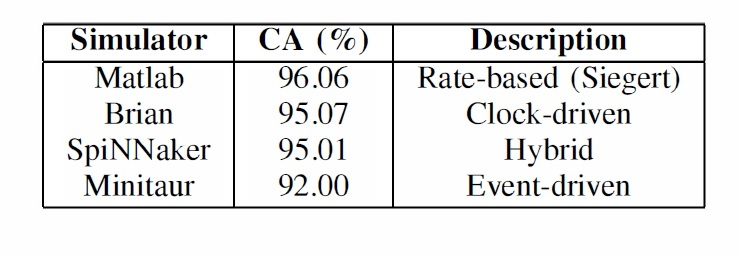
\includegraphics[width=\columnwidth,clip=true]{pics/Accuracy.jpg}}
        \caption{Classification Accuracy}\label{fig:SpiNNaker_results}
      \end{subfigure}%
      \begin{subfigure}{0.5\columnwidth}
        \centering
        {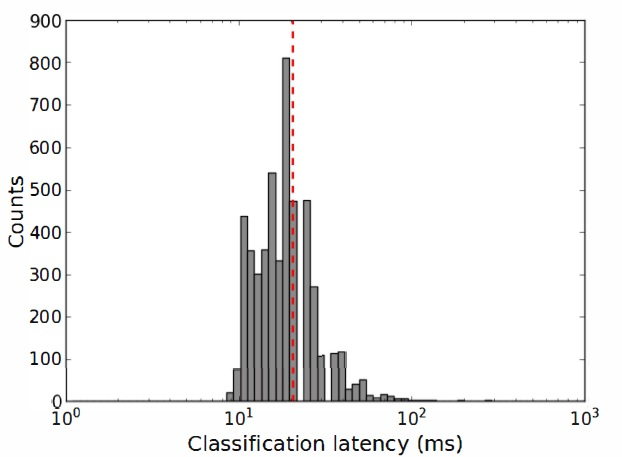
\includegraphics[width=0.9\columnwidth,clip=true]{pics/Latencies.jpg}}
        \caption{Μέση καθυστέρηση}\label{fig:Spinnaker_time}
      \end{subfigure}
      \caption{Επιδόσεις DBN στο SpiNNaker}
    \end{figure}

  \end{subsection}

  \begin{subsection}{BrainScaleS Project (BSS)}
    Στα πλαίσια του BrainScales Project δημιουργήθηκε το Heidelberg Neuromorphic Computing Platform. Πρόκειται για ένα mixed-signal υπολογιστικό σύστημα που δίνει τη δυνατότητα προσομοίωσης νευρομορφικών μοντέλων. Αυτό σημαίνει ότι τα chip είναι αναλογικά, ενώ η επικοινωνία τους γίνεται με ψηφιακό τρόπο.

    \subsubsection{Αρχιτεκτονική Συστήματος}

    Το BrainScaleS αποτελείται από ένα cluster για την είσοδο και την έξοδο των δεδομένων και ένα νευρομορφικό σύστημα. Πυρήνας αυτού του συστήματος είναι το HICANN (High Input Count Analog Neural Network) Chip. Κάθε HICANN μπορεί να προσομοιώσει μέχρι και 512 νευρώνες τύπου Adaptive Exponential που δέχονται είσοδο από 2 ομάδες των 256 συνάψεων.\\
    To σύστημα χρησιμοποιεί wafer-scale integration, δηλαδή τα διαφορετικά chip πάνω στο wafer δε κόβονται σε dies, αλλά συνδέονται μεταξύ τους πάνω στο wafer. Στην εικόνα \eqref{fig:wafer} παρατηρούμε το κάτω mounting, ένα προστατευτικό ceil ring, το wafer πυριτίου που περιέχει τα αναλογικά κυκλώματα, τη motherboard πάνω από το wafer και το πάνω mounting. Η motherboard παρέχει τη διεπαφή μεταξύ του wafer και εξωτερικών FPGAs που χρησιμοποιούνται για την επικοινωνία μεταξύ νευρώνων σε διαφορετικά wafer.\\
    \begin{figure}[H]
      \centering%
      {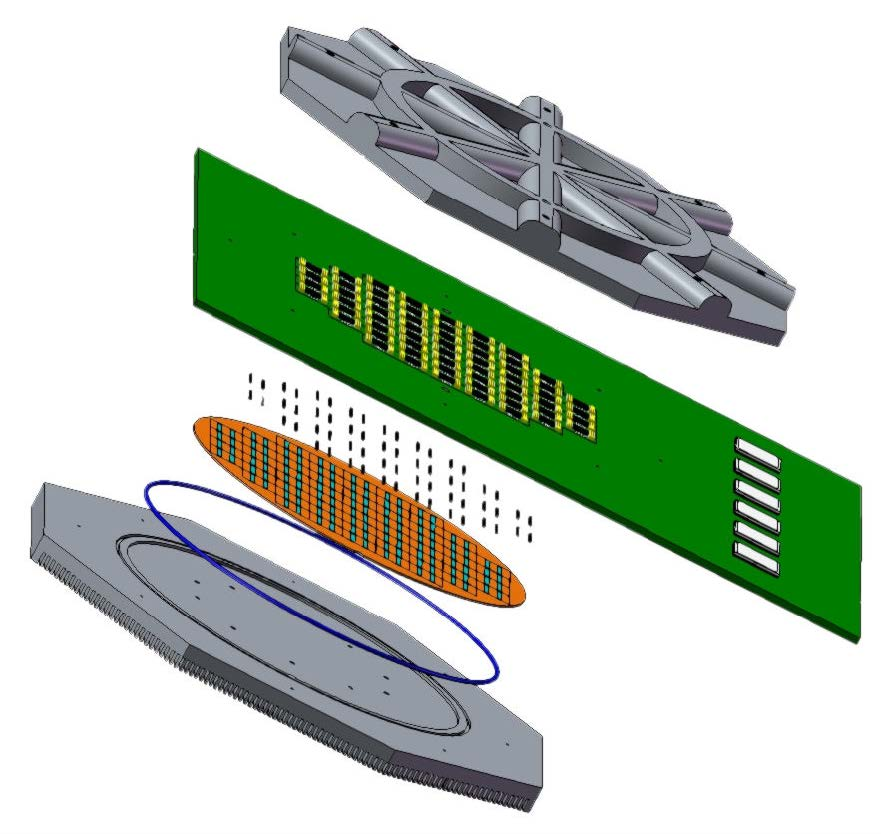
\includegraphics[width=0.3\columnwidth,clip=true]{pics/wafer.jpg}}
      \caption{Wafer συστήματος BrainScales} \label{fig:wafer}
    \end{figure}
    Κάθε wafer περιέχει 384 HICANN chips και μπορεί να μοντελεοποιήσει $200\cdot10^3$ νευρώνες AdEx με 45 εκατομμύρια συνάψεις. Το σημερινό σύστημα αποτελείται από 20 πλήρως συνδεδεμένα wafer.\\
    To wafer χωρίζεται σε reticles, καθένα από τα οποία περιέχει 8 HICANN chips (εικόνα \eqref{fig:reticles}. Τα ANC που σημειώνονται είναι ένας διαφορετικός όρος για το HICANN. Για να επικοινωνούν τα διαφορετικά HICANNs απαιτείται ένα πυκνό δικτύωμα από οριζόντια και κάθετα wires. Αυτό για ιστορικούς λόγους ονομάζεται Layer 1 routing. Λόγω κατασκευαστικών περιορισμών, τα wires εκτείνονται μόνο εντός του reticle. Η επικοινωνία μεταξύ διαφορετικών reticles εξασφαλίζεται με post-processing στο wafer δημιουργώντας συνδέσεις σε επίπεδο πάνω από το αρχικό.\\
    \begin{figure}[H]
      \centering%
      {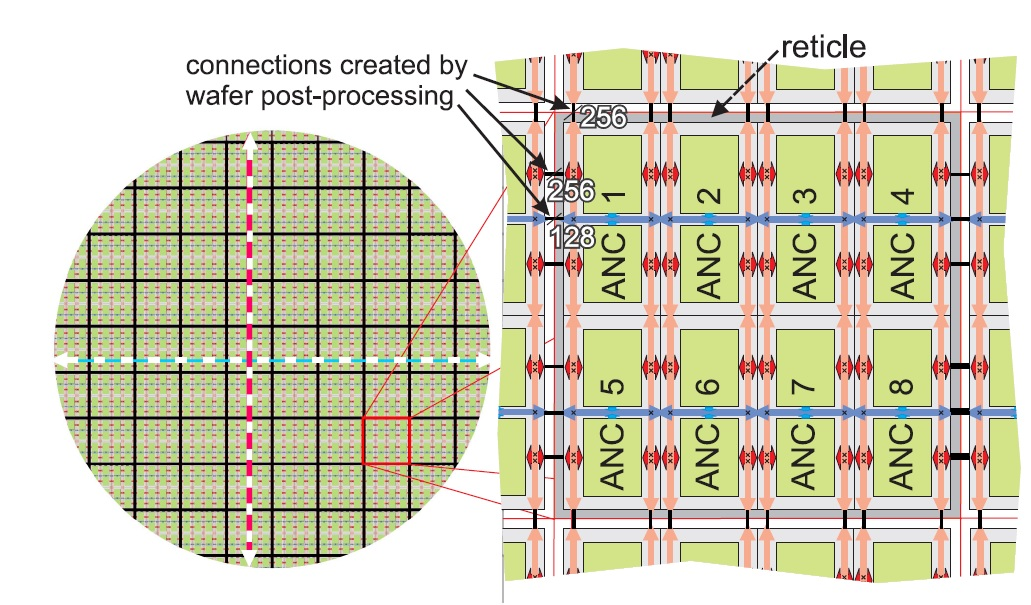
\includegraphics[width=0.5\columnwidth,clip=true]{pics/reticle.jpg}}
      \caption{Δομή και διασυνδέσεις ενός reticle} \label{fig:reticles}
    \end{figure}
    Τα κύρια components του HICANN δίνονται στο σχήμα \eqref{fig:HICANN}. Ο πυρήνας του είναι χωρισμένος σε πάνω και κάτω μέρος, με 256 κυκλώματα «μεμβράνης» σε κάθε πλευρά. Αυτά χρησιμοποιούνται για τα μοντέλα των νευρώνων που θέλουμε να υλοποιήσουμε και ανάλογα με την πολυπλοκότητα μπορεί να υπάρχουν περισσότερα membranes/neuron. Αυτή η ομαδοποίηση των κυκλωμάτων μεμβράνης γίνεται μέσω του Neuron Builder. Η είσοδος των spikes πραγματοποιείται μέσω των synapse drivers που χωρίζονται σε 4 ομάδες στο πάνω και κάτω μέρος. Κάθε spike μεταφέρει μια πληροφορία 6 bits, εκ των οποίων τα δύο πρώτα χρησιμοποιούνται για να επιλεχτεί κάποιο τα 4 strobe lines (που φαίνονται στη μεγέθυνση). Κάθε strobe έχει μια χρονική διάρκεια παλμού $\tau_{STDF}$ που μπορεί να καθορίζεται και από τους learning αλγορίθμους. Τα υπόλοιπα 4 bit μεταφέρονται στο εσωτερικό της διάταξης και αξιοποιούνται στο κομμάτι των συνάψεων.\\
    \begin{figure} [H]
      \centering%
      \begin{subfigure}{0.5\columnwidth}
        {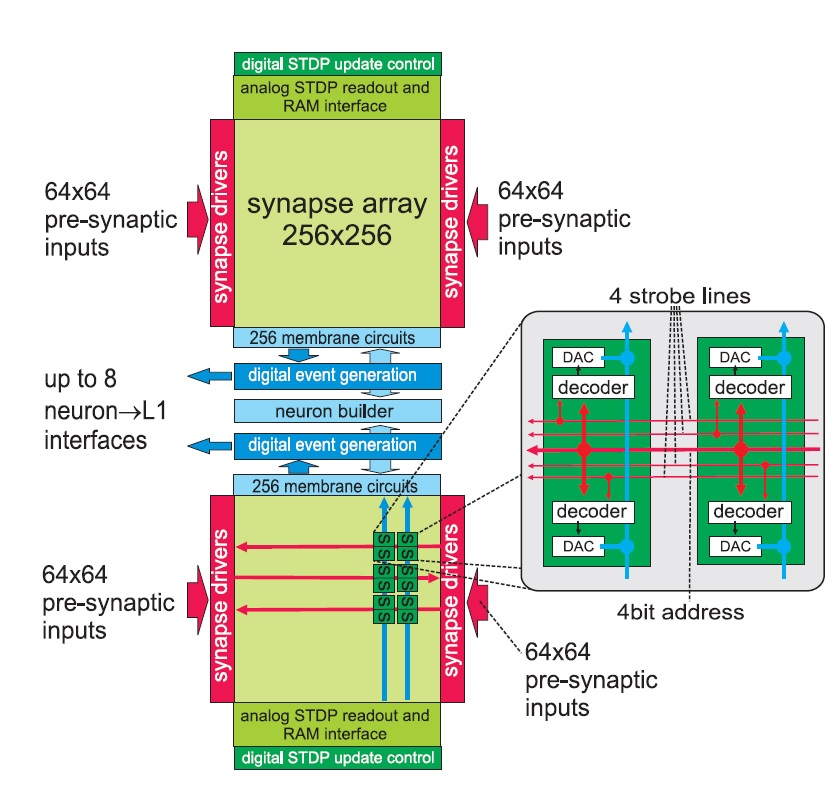
\includegraphics[width=\columnwidth,clip=true]{pics/insideHICANN.jpg}}
        \caption{Δομή HICANN}\label{fig:HICANN}
      \end{subfigure}%
      \begin{subfigure}{0.5\columnwidth}
        \centering
        {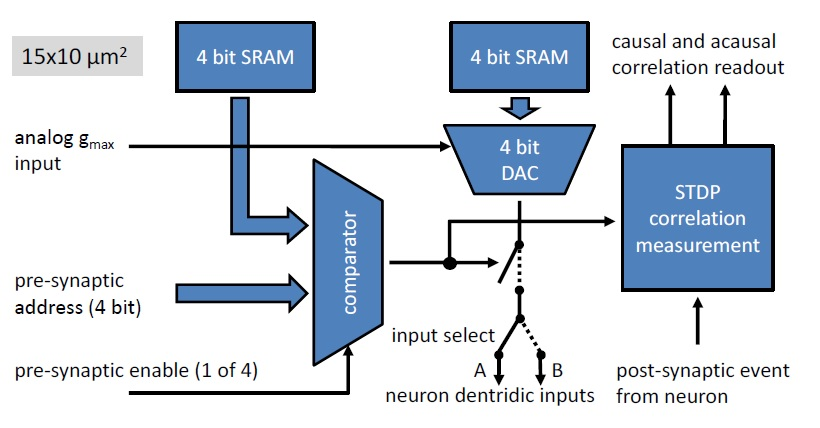
\includegraphics[width=0.9\columnwidth,clip=true]{pics/synapses.jpg}}
        \caption{Δομή Σύναψης}\label{fig:Synapses}
      \end{subfigure}
      \caption{Εσωτερικό HICANN chip}
    \end{figure}
    Κάθε σύναψη είναι συνδέεται με ένα συγκεκριμένο strobe line. To βάρος των συνάψεων αποθηκεύεται σε μια 4bit SRAM και μέσω ενός DAC μεταφράζεται σε επίπεδο ρεύματος, όπως φαίνεται στο σχήμα \eqref{fig:Synapses} και πολλαπλασιάζεται με ένα παράγοντα αγωγιμότητας $g_{max}$ που επίσης μπορεί να μεταβάλλεται. Επιπρόσθετα, κάθε σύναψη περιέχει και ένα address σε μια άλλη 4bit SRAM η οποία συγκρίνεται με τα 4 από τα 6 εναπομείναντα bits που περιέχει το spike. Εφόσον συμπίπτουν, για όσο διάστημα $\tau_{STDF}$ διαρκεί ο παλμός του stobe που μπαίνει στο pre-synaptic enable του συγκριτή θα έχουμε input στο δενδρίτη της μεμβράνης. Συνοψίζοντας, έχουμε ένα spike διάρκειας $\tau_{STDF}$ και πλάτους $g_{max}\cdot weight$ που μας δίνει ένα πολύ καλό resolution σε ότι αφορά τα weights. Τέλος, υπάρχουν 2 inputs A και B στο κύκλωμα μεμβράνης που μπορούν να επιλέγονται με έναν multiplexer. Το ένα input μπορεί να χρησιμοποιείται ως excitatory και το άλλο ως inhibitory, χρήσιμο στοιχείο για τους HTM αλγορίθμους.\\
    Στη συνέχεια, θα δούμε ένα παράδειγμα επικοινωνίας μεταξύ δύο νευρώνων σε διαφορετικά HICANN chips (εικόνα \eqref{fig:communication}). O priority encoder χρησιμοποιείται για να επιλέξει το neuron με τη μεγαλύτερη προτεραιότητα, ενώ από τον serializer παίρνουμε τη σειριακή ψηφιακή πληροφορία. Στο άκρο κάθε reticle ενσωματώνεται ένας repeater για να αποκαταστήσει το πλάτος και τη διάρκεια του σήματος. Επίσης, σε κάθε διασταύρωση οριζόντιων και κατακόρυφων L1 buses υπάρχουν crossbar switches ώστε το spike να φτάσει τελικά στον προορισμό του περνώντας από διαφορετικά reticles και να αποκωδικοποιηθεί, όπως περιγράφηκε από τον driver του HICANN του δέκτη. Σε περίπτωση που θέλουμε να περάσουμε σε άλλο wafer, θα πρέπει να μεταδοθεί η πληροφορία στη motherboard και με συνδέσεις Ethernet 10 Gbps και FPGA να εισέλθει σε άλλα wafers.\\
    \begin{figure}[H]
      \centering%
      {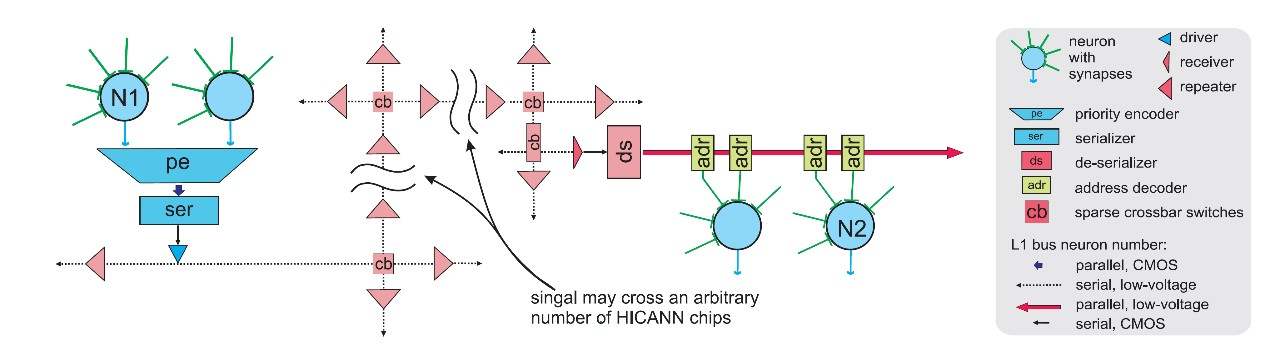
\includegraphics[width=\columnwidth,clip=true]{pics/communication.jpg}}
      \caption{Επικοινωνία HICANNs} \label{fig:communication}
    \end{figure}

    \subsubsection{Adaptive Exponential (AdEx) Neuron Model}

    Το σύστημα χρησιμοποιεί το μοντέλο AdEx που υλοποιεί έναν spiking νευρώνα. Αυτό το μοντέλο περιγράφεται από δύο μεταβλητές: το δυναμικό μεμβράνης και το adaptation μέσω ενός συστήματος διαφορικών εξισώσεων. Στην ύπαρξη DC input, το δυναμικό της μεμβράνης αυξάνεται και μόλις γίνει το spike πέφτει στη μηδενική κατάσταση. Το adaptation αναπαριστά το threshold και η αύξηση του κάνει τα spikes όλο και πιο αραιά στο χρόνο (εικόνα \eqref{fig:AdEx}).
    \begin{figure}[H]
      \centering%
      {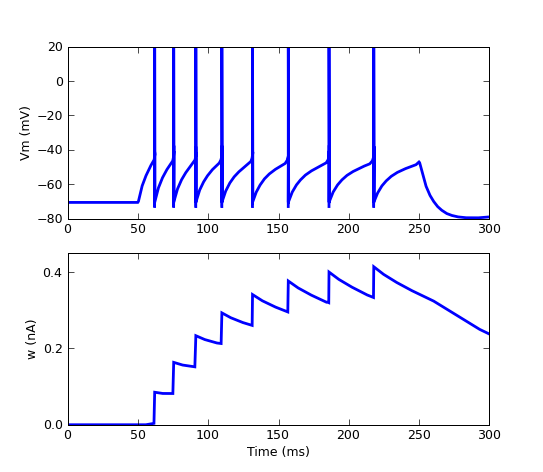
\includegraphics[width=0.45\columnwidth,clip=true]{pics/adex.jpg}}
      \caption{Μοντέλο AdEx Neuron} \label{fig:AdEx}
    \end{figure}
    Στις διαφορικές του μοντέλου υπάρχουν αρκετές παράμετροι που μπορούν να πάρουν κατάλληλες τιμές για να υλοποιήσουν διαφορετικές βιολογικές λειτουργίες. Σημαντικό χαρακτηριστικό αποτελεί ότι το rise time εξαρτάται από την στάθμη της τάσης εισόδου.

    \subsubsection{Υλοποιήσεις λειτουργιών HTM στο BSS}

    Τα δύο βασικότερα λειτουργικά μέρη του HTM είναι ο spatial pooler και ο temporal pooler. Στην εικόνα \eqref{fig:Spatial_hardware} παρατηρούμε την υλοποίηση του spatial pooler, όπου διαφορετικά neurons (με κόκκινο χρώμα) δέχονται μια είσοδο. Όποια έχουν το μεγαλύτερο overlap πυροδοτούνται πρώτα, λόγω μικρότερου rise time. Το inhibition cell  (Ι) δέχεται είσοδο από όλα τα cells και λειτούργει σαν counter. Μόλις ξεπεραστεί ένα κατώφλι ενεργών cells αποτρέπει τα υπόλοιπα από το να πυροδοτηθούν. Με αυτό τον τρόπο πετυχαίνει να διατηρεί το sparsity της SDR αναπαράστασης. Επιπλέον, έχει τη δυνατότητα σε στιγμές υψηλής συνολικής δραστηριότητας να σταθεροποιεί το σύστημα αυξάνοντας όλους τους χρόνους ανόδου κατά μια σταθερή ποσότητα.\\
    \begin{figure}[H]
      \centering%
      {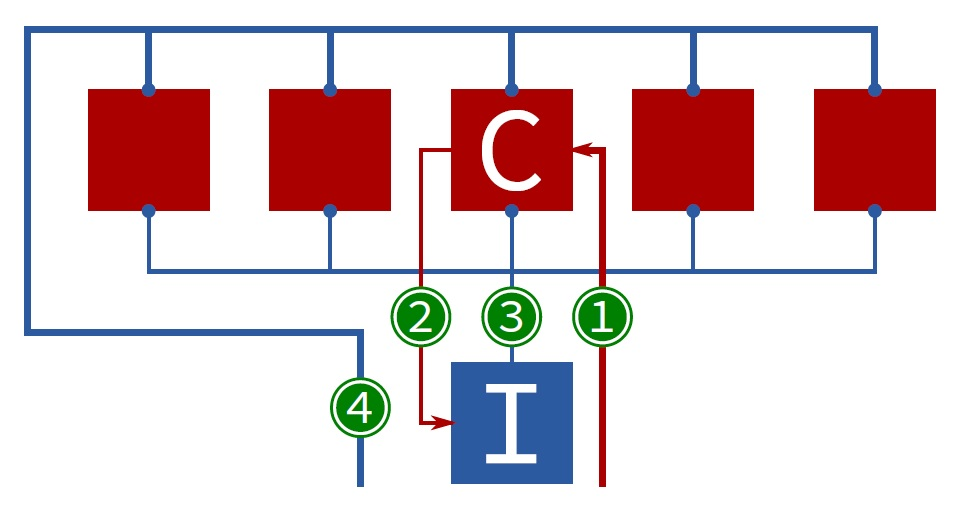
\includegraphics[width=0.45\columnwidth,clip=true]{pics/spatial_hardware.jpg}}
      \caption{Υλοποίηση Spatial Pooler} \label{fig:Spatial_hardware}
    \end{figure}

    O temporal pooler προσθέτει το στοιχείο της πρόβλεψης και της ακολουθιακής μνήμης στο HTM. Στα πλαίσια του BSS ένα neuron ενός minicolumn απαιτεί μια τριάδα από cells (D,I,S), όπως στην εικόνα \eqref{fig:Temporal_hardware}. Όλα τα neurons του minicolumn μοιράζονται το ίδιο perceptive field μέσω του στοιχείου P. Στην πραγματικότητα το P αποτελεί μέρος του spatial pooler που περιγράφηκε στην προηγούμενη παράγραφο. Σε περίπτωση που δεν υπάρχει predicted cell και το minicolumn λάβει επαρκή είσοδο, μέσω του P θα ενεργοποιηθούν όλα τα σώματα S. Αντίθετα, αν υπάρχει ένα predicted cell, το I και D cell είναι σε μια depolarized κατάσταση. Μόλις έρθει input το I θα εμποδίσει μέσω inhibitory σήματος την πυροδότηση των υπόλοιπων σωμάτων. Τέλος, για να επιτραπούν πολλαπλές προβλέψεις εντός του minicolumn συνδέεται και το D με το S, ώστε να αναιρέσει στην επίδραση του inhibition σε περίπτωση 2 ή περισσότερων predicted cells.\\
\begin{figure}[H]
  \centering%
  {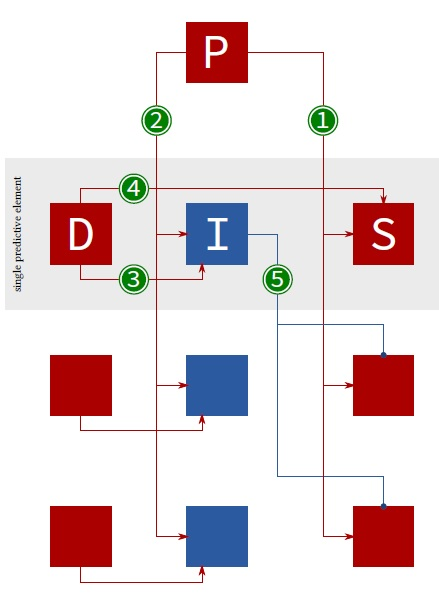
\includegraphics[width=0.4\columnwidth,clip=true]{pics/temporal_hardware.jpg}}
  \caption{Υλοποίηση Temporal Pooler} \label{fig:Temporal_hardware}
\end{figure}
Από τα αποτελέσματα στα σχήματα \eqref{fig:spatial_sim_1} και \eqref{fig:spatial_sim_2} βεβαιώνεται η πολύ καλή λειτουργία του Spatial Pooler που αφενός ενεργοποιεί μόνο τα neurons με το μεγαλύτερο overlap score, αφαιτέρου απεικονίζει όμοιες εισόδους σε όμοια SDR εξόδου. To τελευταίο αποτελεί σημαντική απαίτηση ώστε να διατηρούνται οι συσχετίσεις πληροφορίας στην είσοδο και την έξοδο.
\begin{figure} [H]
  \centering%
  \begin{subfigure}{0.5\columnwidth}
    {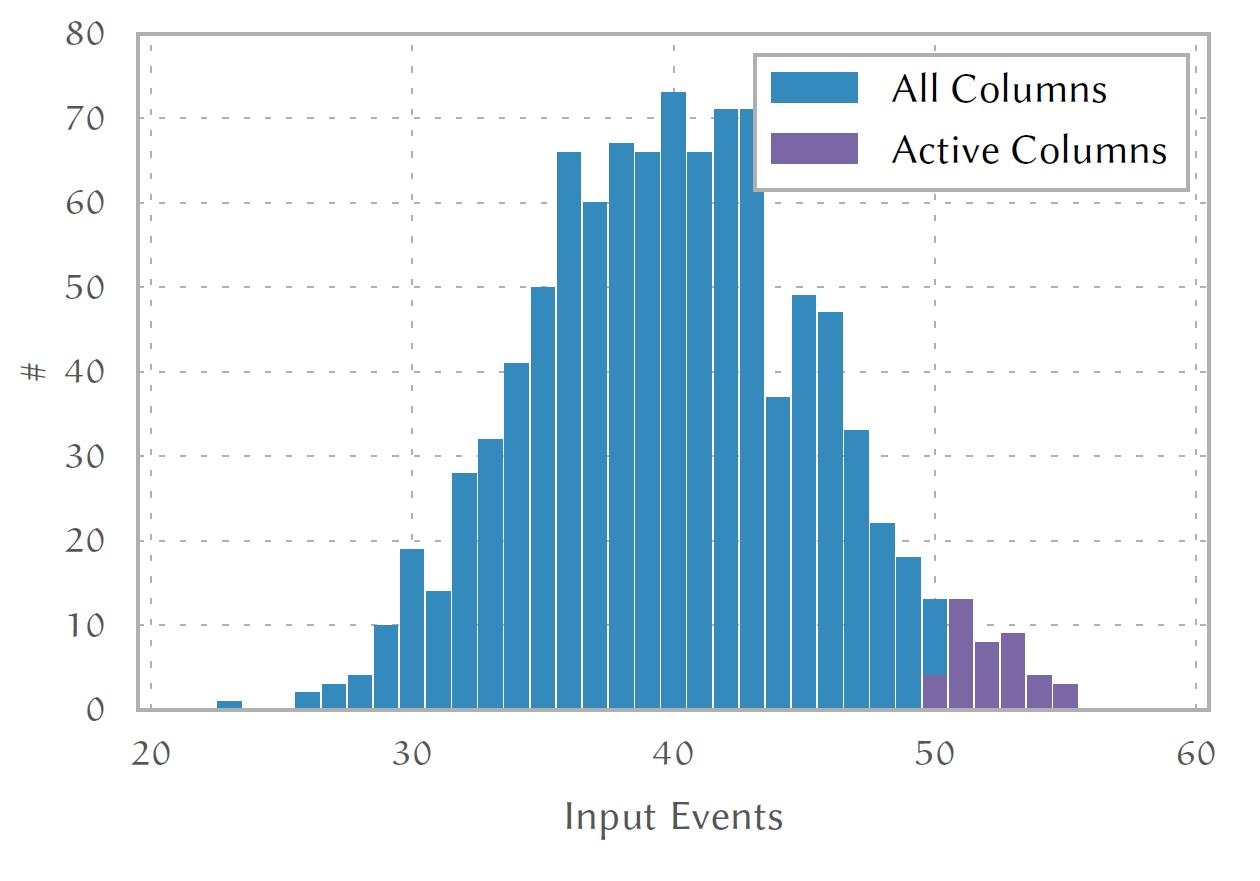
\includegraphics[width=\columnwidth,clip=true]{pics/spatialsim1.jpg}}
    \caption{Ενεργοποίηση νευρώνων} \label{fig:spatial_sim_1}
  \end{subfigure}%
  \begin{subfigure}{0.5\columnwidth}
    \centering
    {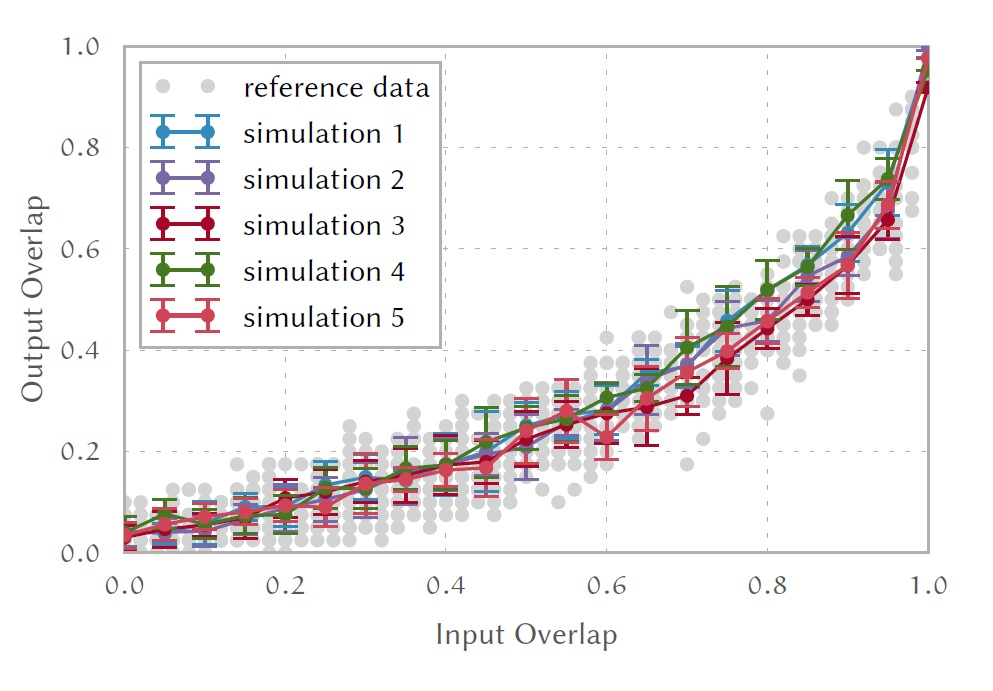
\includegraphics[width=\columnwidth,clip=true]{pics/spatialsim2.jpg}}
    \caption{Διατήρηση συσχετίσεων πληροφορίας} \label{fig:spatial_sim_2}
  \end{subfigure}
  \caption{Προσομοιώσεις Spatial Pooler στο BSS}
\end{figure}

\end{subsection}
\end{section}

\newpage
\nocite{*}
\begin{section}{Βιβλιογραφία}
	\printbibliography
\end{section}

\end{document}
